\chapter{Result}
104 Borehole Log Data of 31 locations inside Kathmandu and Lalitpur district areas were taken into consideration. The results were obtained after calculating Bearing Capacity at 1.5m, 3m, and 4.5m depth by shear criteria using Terzaghi, Meyerhof, Hansen, Vesic and Teng methods and Plaxis2D software and by deflection criteria using Bowels, Teng, Peck, Meyerhof methods and Plaxis2D software. The median value of those methods are taken and mapped for those depths. Liquefaction Potential Index of the area is also mapped. While mapping, to make the map uniform and consistent and for better results in interpolation, outlier values having too small or high values are disregarded.
\pagebreak

\section{Location Table}
\begin{table}[!h]
\caption{Location Table}
\begin{tabularx}{\textwidth}{ | l | p{0.6\textwidth} | X | X | }
\hline
 \textbf{S.N.} & \textbf{Location} & \textbf{Latitude} & \textbf{Longitude} \\
\hline
 1 & Rastriya Banijya Bank: Thapathali, Kathmandu & 27.65586 & 85.30645 \\
 2 & Building Complex: Anamnagar, Kathmandu & 27.69728 & 85.32746 \\
 3 & Building Complex: Bakhundol Lalitpur & 27.68302 & 85.31033 \\
 4 & Hindu vidhypeth: Balkumari, Lalitpur & 27.67114 & 85.33793 \\
 5 & DI Skin Health and Referral Center (P). Ltd.: Bansbari, Kathmandu & 27.73704 & 85.33354 \\
 6 & Building: Bhaisipati, Lalitpur & 27.64805 & 85.29596 \\
 7 & Brihaspati Vidyasadan School: Gahanapokhari, Kathmandu & 27.71425 & 85.32957 \\
 8 & Green Hill City (P). Ltd. : Mulpani, Kathamndu  & 27.71577 & 85.38647 \\
 9 & Building Site: Itachhe tol, Bhaktapur & 27.67284 & 85.42261 \\
 10 & Buddha Air (P). Ltd. : Jawalakhel, Lalitpur  & 27.67357 & 85.31187 \\
 11 & Tamrakar Samaj: Jawalakhel & 27.67475 & 85.31220 \\
 12 & Tangal, Kathmandu & 27.72009 & 85.32626 \\
 13 & Harihar Bhavan, Lalitpur & 27.68047 & 85.31111 \\
 14 & Janamaitri Campus: Kuleswore, Kathmandu & 27.69173 & 85.29005 \\
 15 & Amrit Science Campus: Lainchour, Kathmandu & 27.71776 & 85.31061 \\
 16 & Mahendra Ratna Campus: Tahachal, Kathmandu & 27.70346 & 85.29821 \\
 17 & Bhatbhateni Supermarket \& Departmental Store: Satdobato, Lalitpur & 27.65712 & 85.32002 \\
 18 & Nepal Mountaineering Association :  Naxal, Nagpokhari Kathmandu  & 27.71303 & 85.32167 \\
 19 & Patanjali Yogpeeth Nepal : Mandikatar, Kathmandu  & 27.74115 & 85.34555 \\
 20 & Mandikhatar, Kathmandu  & 27.73878 & 85.34535 \\
 21 & CIWEC Clinic: Lainchaur, Kathmandu  & 27.72040 & 85.31555 \\
 22 & Vastukala Pharamarsha Nepal : Kupondole, Lalitpur & 27.68376 & 85.31634 \\
 23 & Building: Kupondole, Lalitpur & 27.68628 & 85.31470 \\
 24 & NAST Technology : Khumaltar, Lalitpur & 27.65610 & 85.32768 \\
 25 & Building: Khumaltar, Lalitpur  & 27.64870 & 85.32034 \\
 26 & Building: Kalopul, Pumori, Kathmandu & 27.71183 & 85.33536 \\
 27 & Building Site : Gwarkho, Lalitpur & 27.66601 & 85.32847 \\
 28 & Building: Kumaripati, Lalitpur & 27.67025 & 85.31863 \\
 29 & Building: Kupandole, Lalitpur & 27.68703 & 85.30930 \\
 30 & Nepal Rastra Bank: Thapathali & 27.69023 & 85.31993 \\
 31 & Exam Mega Hall Construction Project : Kirtipur, Kathmandu & 27.68426 & 85.29536 \\
\hline
\end{tabularx}

\end{table}
\pagebreak

\begin{landscape}
\section{Locations map\index{map}}
\begin{figure}[!h]
\centering
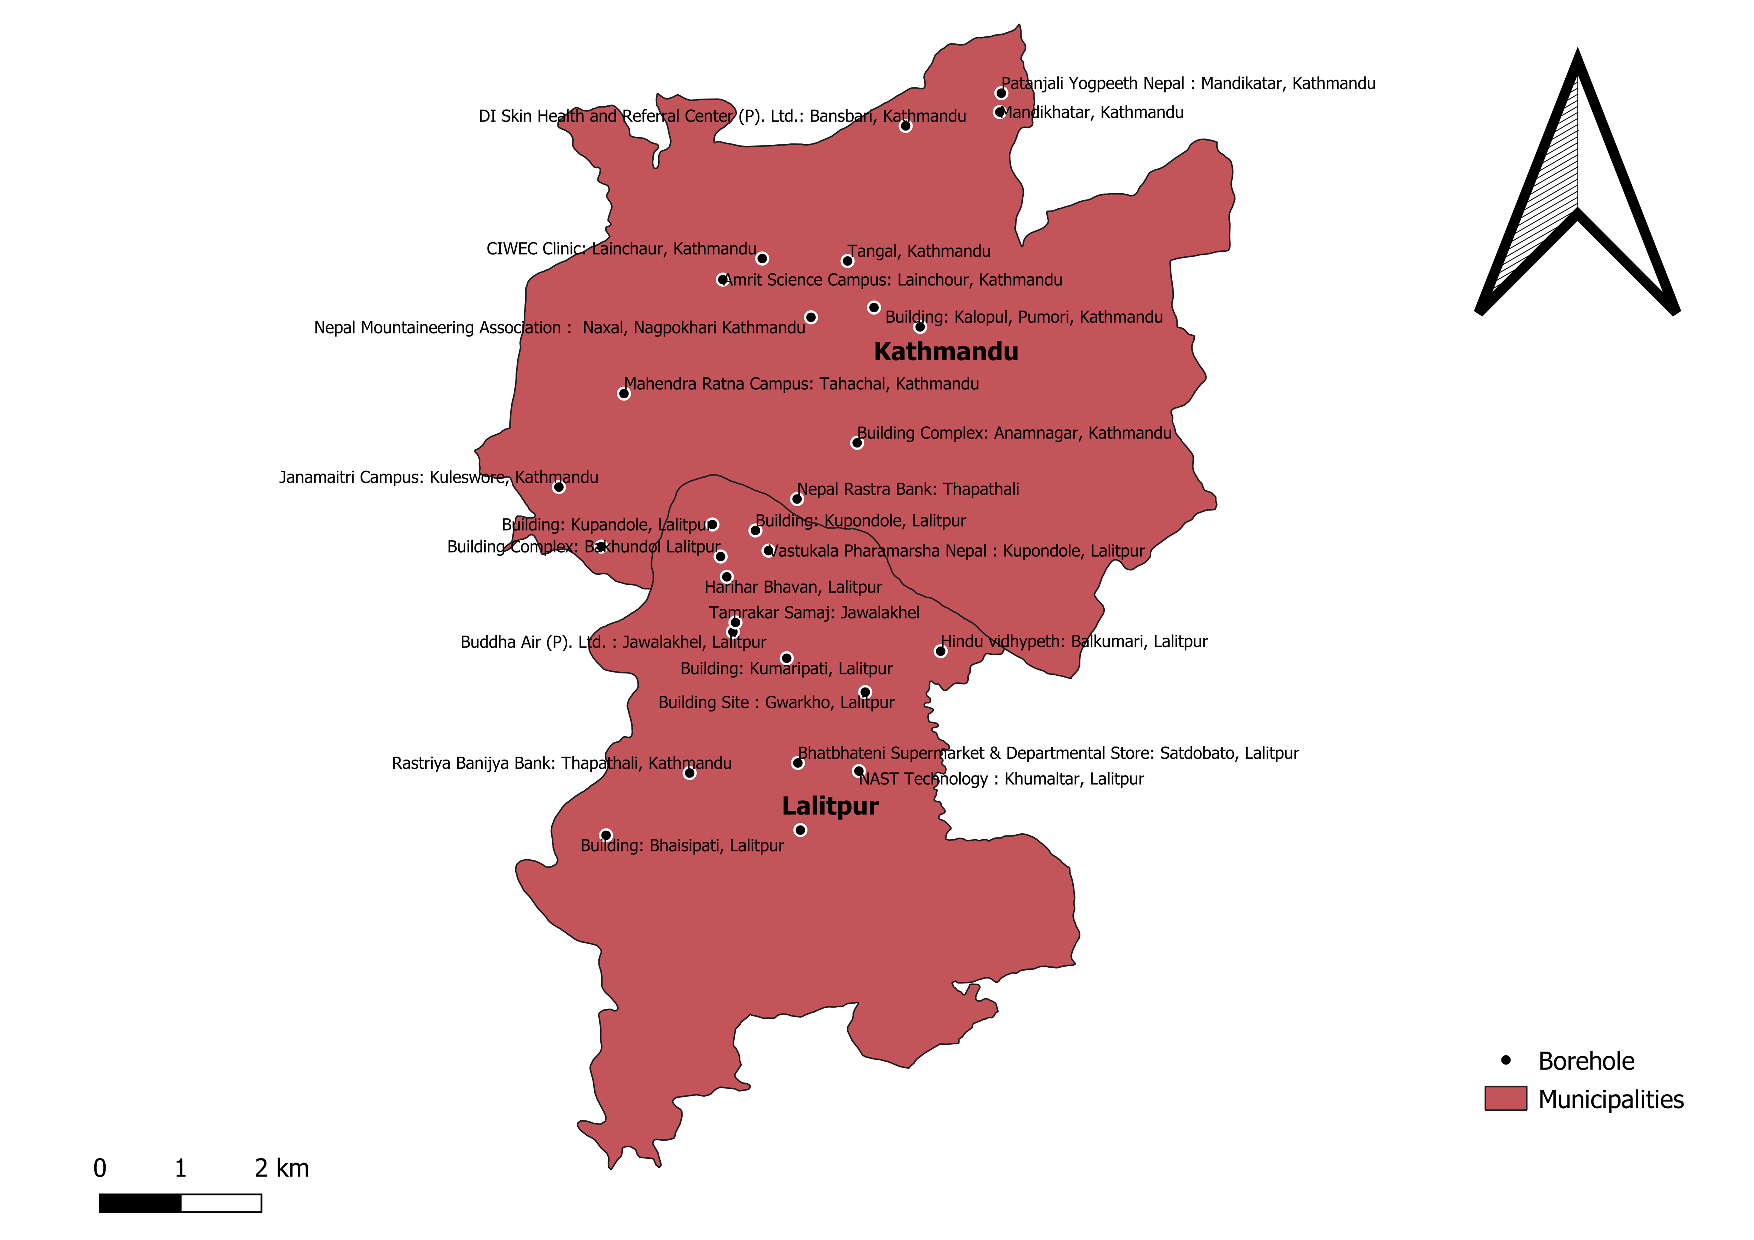
\includegraphics[width=0.8\linewidth, height=0.8\textheight,keepaspectratio]{in/map/Borehole2.png}
\caption{Borehole locations\index{map}}
\end{figure}
\pagebreak
\end{landscape}

\section{Shear Strength Table(kPa)}
\begin{table}[!h]
\caption{Shear Strength Table}
\begin{tabularx}{\textwidth}{ | l | p{0.5\textwidth} | X | X | X | }
\hline
 \textbf{S.N.} & \textbf{Location} & \textbf{1.5m} & \textbf{3.0m} & \textbf{4.5m}\\
\hline
 1 & Thapathali, Kathmandu & 556.783 & 881.966 & 1219.911 \\
 2 & Anamnagar, Kathmandu & 226.203 & 253.102 & 210.010 \\
 3 & Bakhundol Lalitpur & 78.274 & 109.557 & 126.082 \\
 4 & Balkumari, Lalitpur & 347.149 & 705.395 & 497.897 \\
 5 & Bansbari, Kathmandu & 226.203 & 411.124 & 573.964 \\
 6 & Bhaisipati, Lalitpur & 318.034 & 654.486 & 375.495 \\
 7 & Gahanapokhari, Kathmandu & 160.596 & 211.665 & 408.875 \\
 8 & Mulpani, Kathamndu  & 85.764 & 155.830 & 738.492 \\
 9 & Itachhe tol, Bhaktapur & 103.915 & 141.288 & 161.811 \\
 10 & Jawalakhel, Lalitpur  & 295.379 & 525.479 & 351.012 \\
 11 & Jawalakhel & 154.538 & 188.042 & 218.952 \\
 12 & Tangal, Kathmandu & 818.280 & 1500.181 & 1701.000 \\
 13 & Harihar Bhavan, Lalitpur & 678.380 & 862.325 & 1080.162 \\
 14 & Kuleswore, Kathmandu & 258.687 & 440.825 & 510.316 \\
 15 & Lainchour, Kathmandu & 427.627 & 1031.251 & 1534.093 \\
 16 & Tahachal, Kathmandu & 213.742 & 278.658 & 324.310 \\
 17 & Satdobato, Lalitpur & 664.956 & 750.835 & 216.900 \\
 18 & Naxal, Nagpokhari Kathmandu  & 661.987 & 1034.337 & 1088.942 \\
 19 & Mandikatar, Kathmandu  & 216.255 & 558.979 & 750.723 \\
 20 & Mandikhatar, Kathmandu  & 166.394 & 374.942 & 819.365 \\
 21 & Lainchaur, Kathmandu  & 961.112 & 1349.100 & 1269.905 \\
 22 & Kupondole, Lalitpur & 197.198 & 707.709 & 1129.132 \\
 23 & Kupondole, Lalitpur & 177.101 & 213.827 & 248.214 \\
 24 & Khumaltar, Lalitpur & 130.857 & 158.837 & 179.932 \\
 25 & Khumaltar, Lalitpur  & 113.986 & 140.911 & 169.485 \\
 26 & Kalopul, Pumori, Kathmandu & 702.484 & 1078.437 & 1160.662 \\
 27 & Gwarkho, Lalitpur & 101.891 & 139.931 & 175.822 \\
 28 & Kumaripati, Lalitpur & 976.011 & 1705.445 & 1978.329 \\
 29 & Kupandole, Lalitpur & 107.883 & 127.698 & 152.281 \\
 30 & Thapathali & 381.822 & 577.350 & 761.849 \\
 31 & Kirtipur, Kathmandu & 363.008 & 713.392 & 1008.880 \\
\hline
\multicolumn{2}{|X|}{\mbox{Mean($\overline{x}$)}} & 350.726 & 580.094 & 682.026 \\
\multicolumn{2}{|X|}{\mbox{Standard deviation($\sigma$)}} & 262.236 & 428.627 & 505.678 \\
\multicolumn{2}{|X|}{\mbox{Minimum($x_{min}$)}} & 78.274 & 109.557 & 126.082 \\
\multicolumn{2}{|X|}{\mbox{Maximum($x_{max}$)}} & 976.011 & 1705.445 & 1978.329 \\
\hline
\end{tabularx}

\end{table}
\pagebreak

\begin{landscape}
\section{1.5m Bearing Capacity(shear)\index{map}}
\begin{figure}[!hbt]
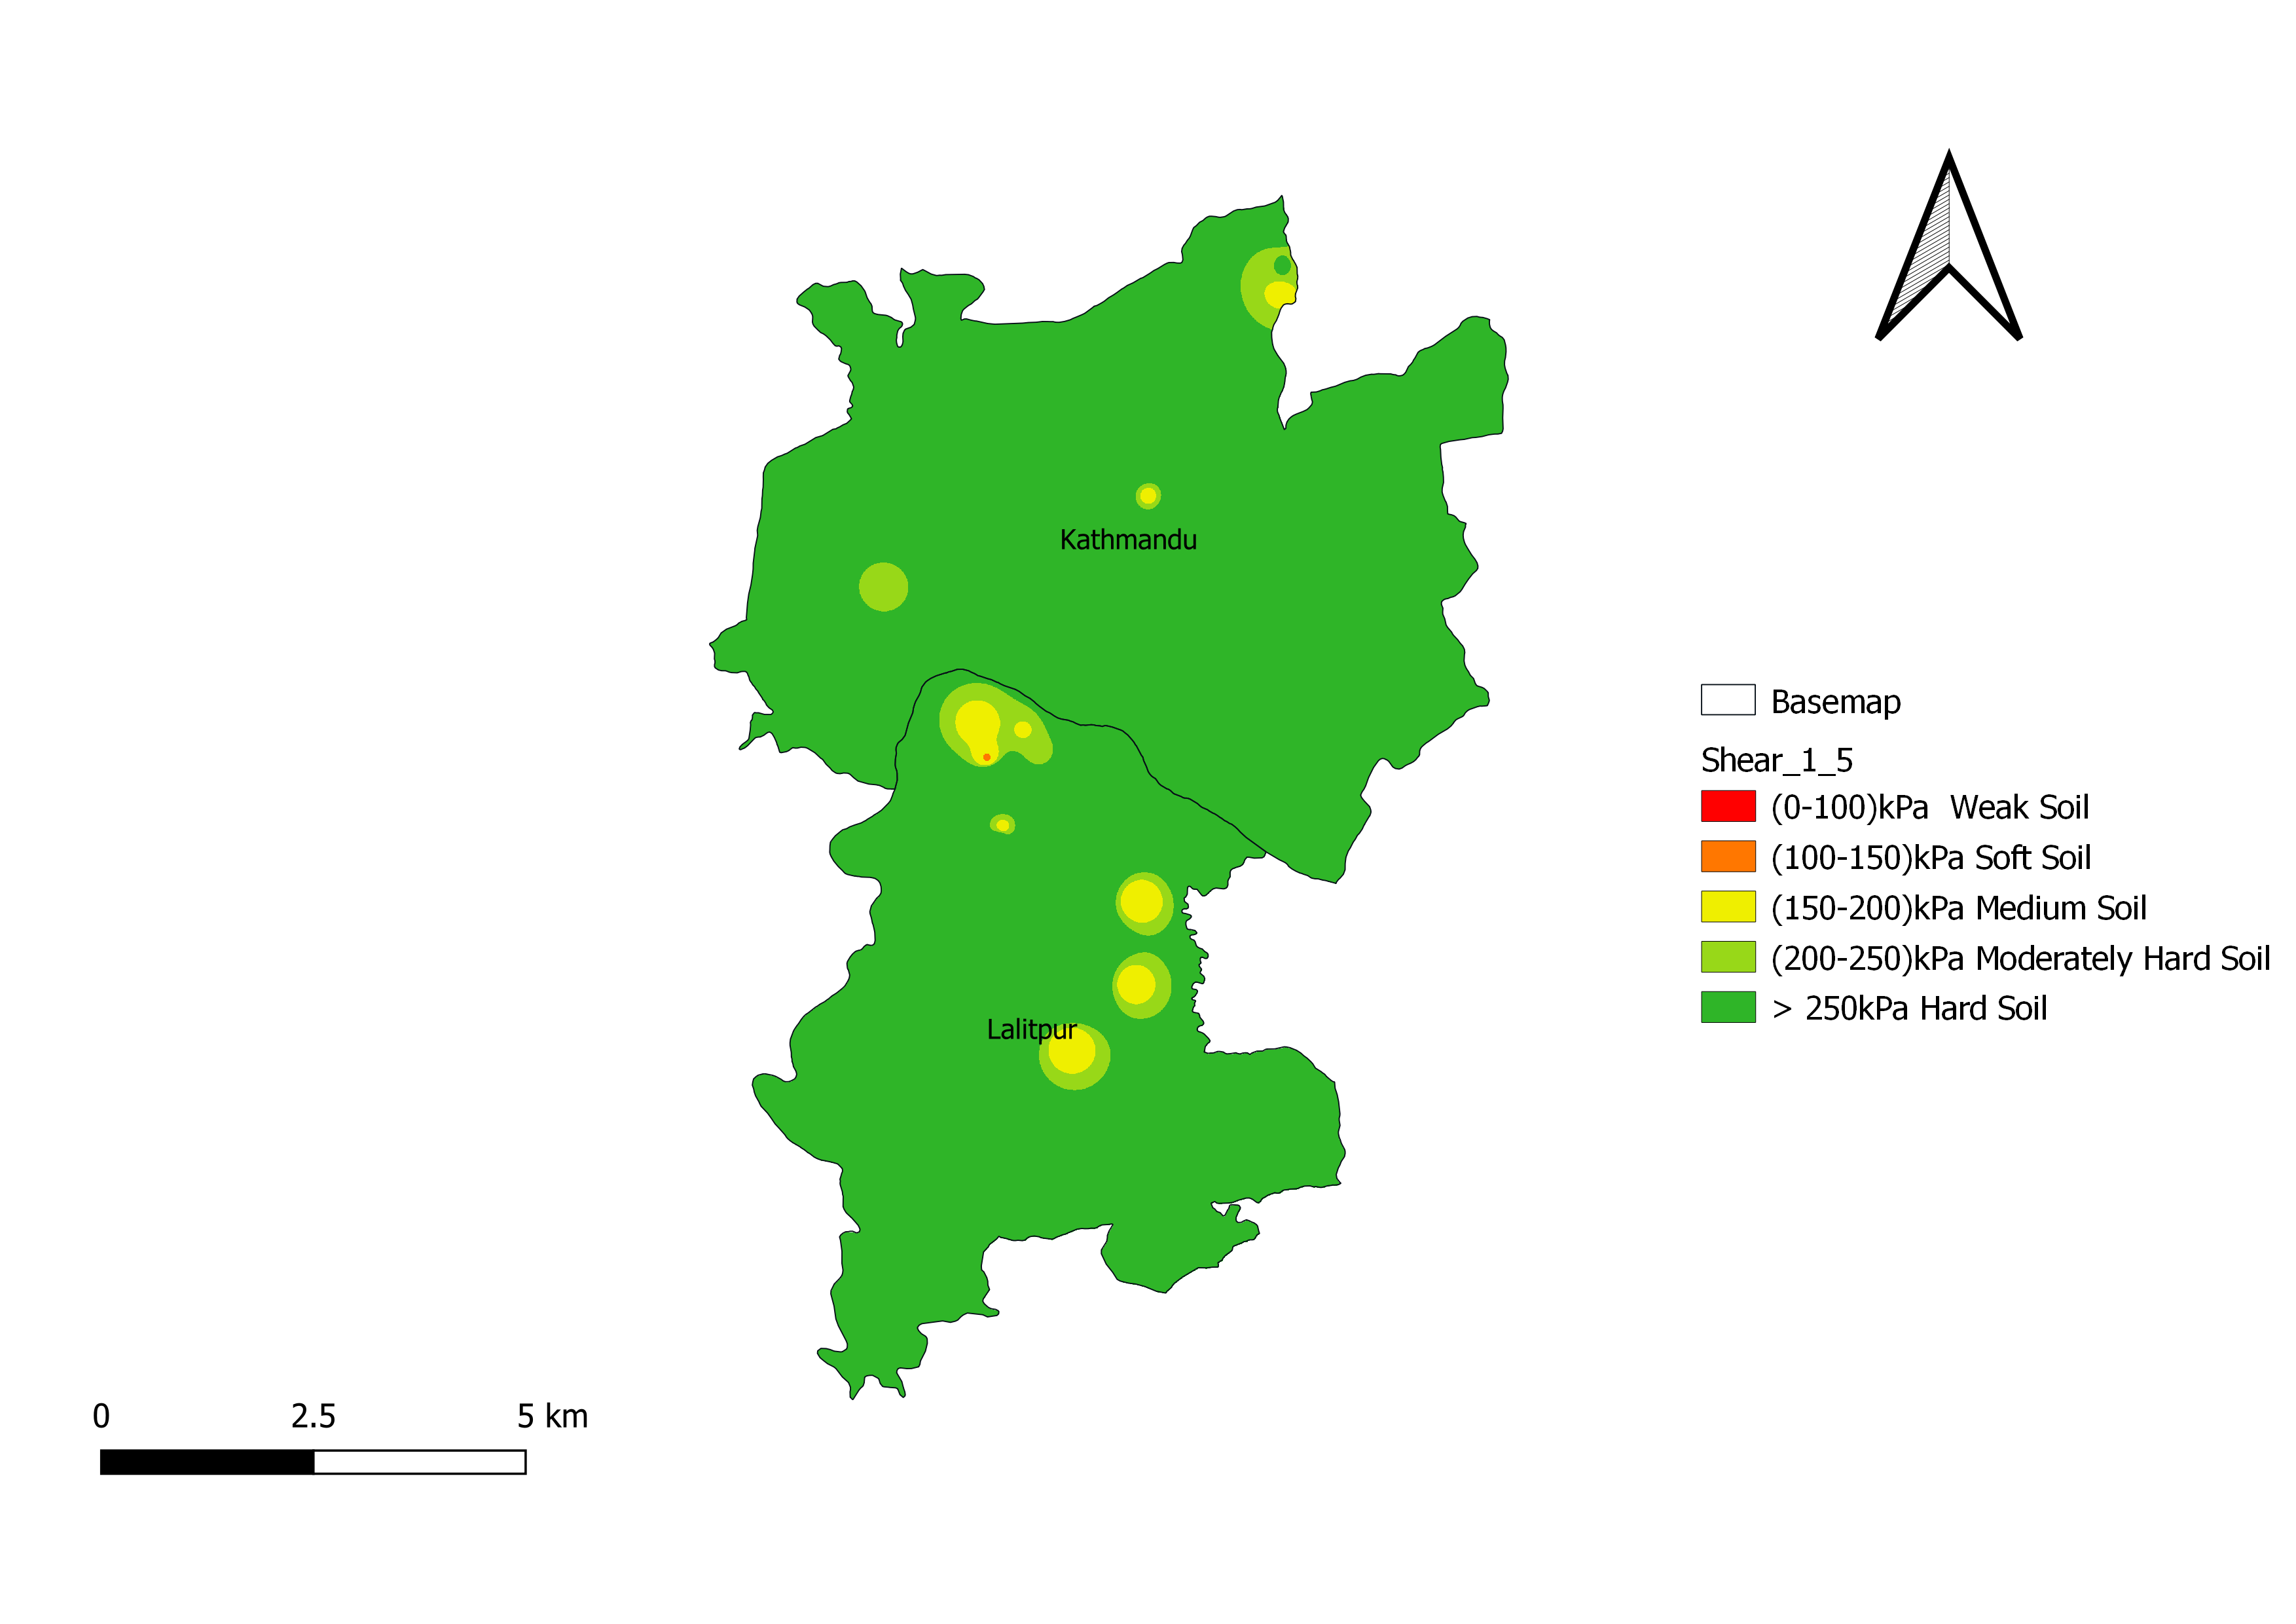
\includegraphics[width=0.8\linewidth, height=0.8\textheight,keepaspectratio]{in/map/Shear_1_5.png}
\caption{BC at 1.5m depth}
\end{figure}
\pagebreak
\end{landscape}

\begin{landscape}
\section{3.0m Bearing Capacity(shear)\index{map}}
\begin{figure}[!hbt]
\centering
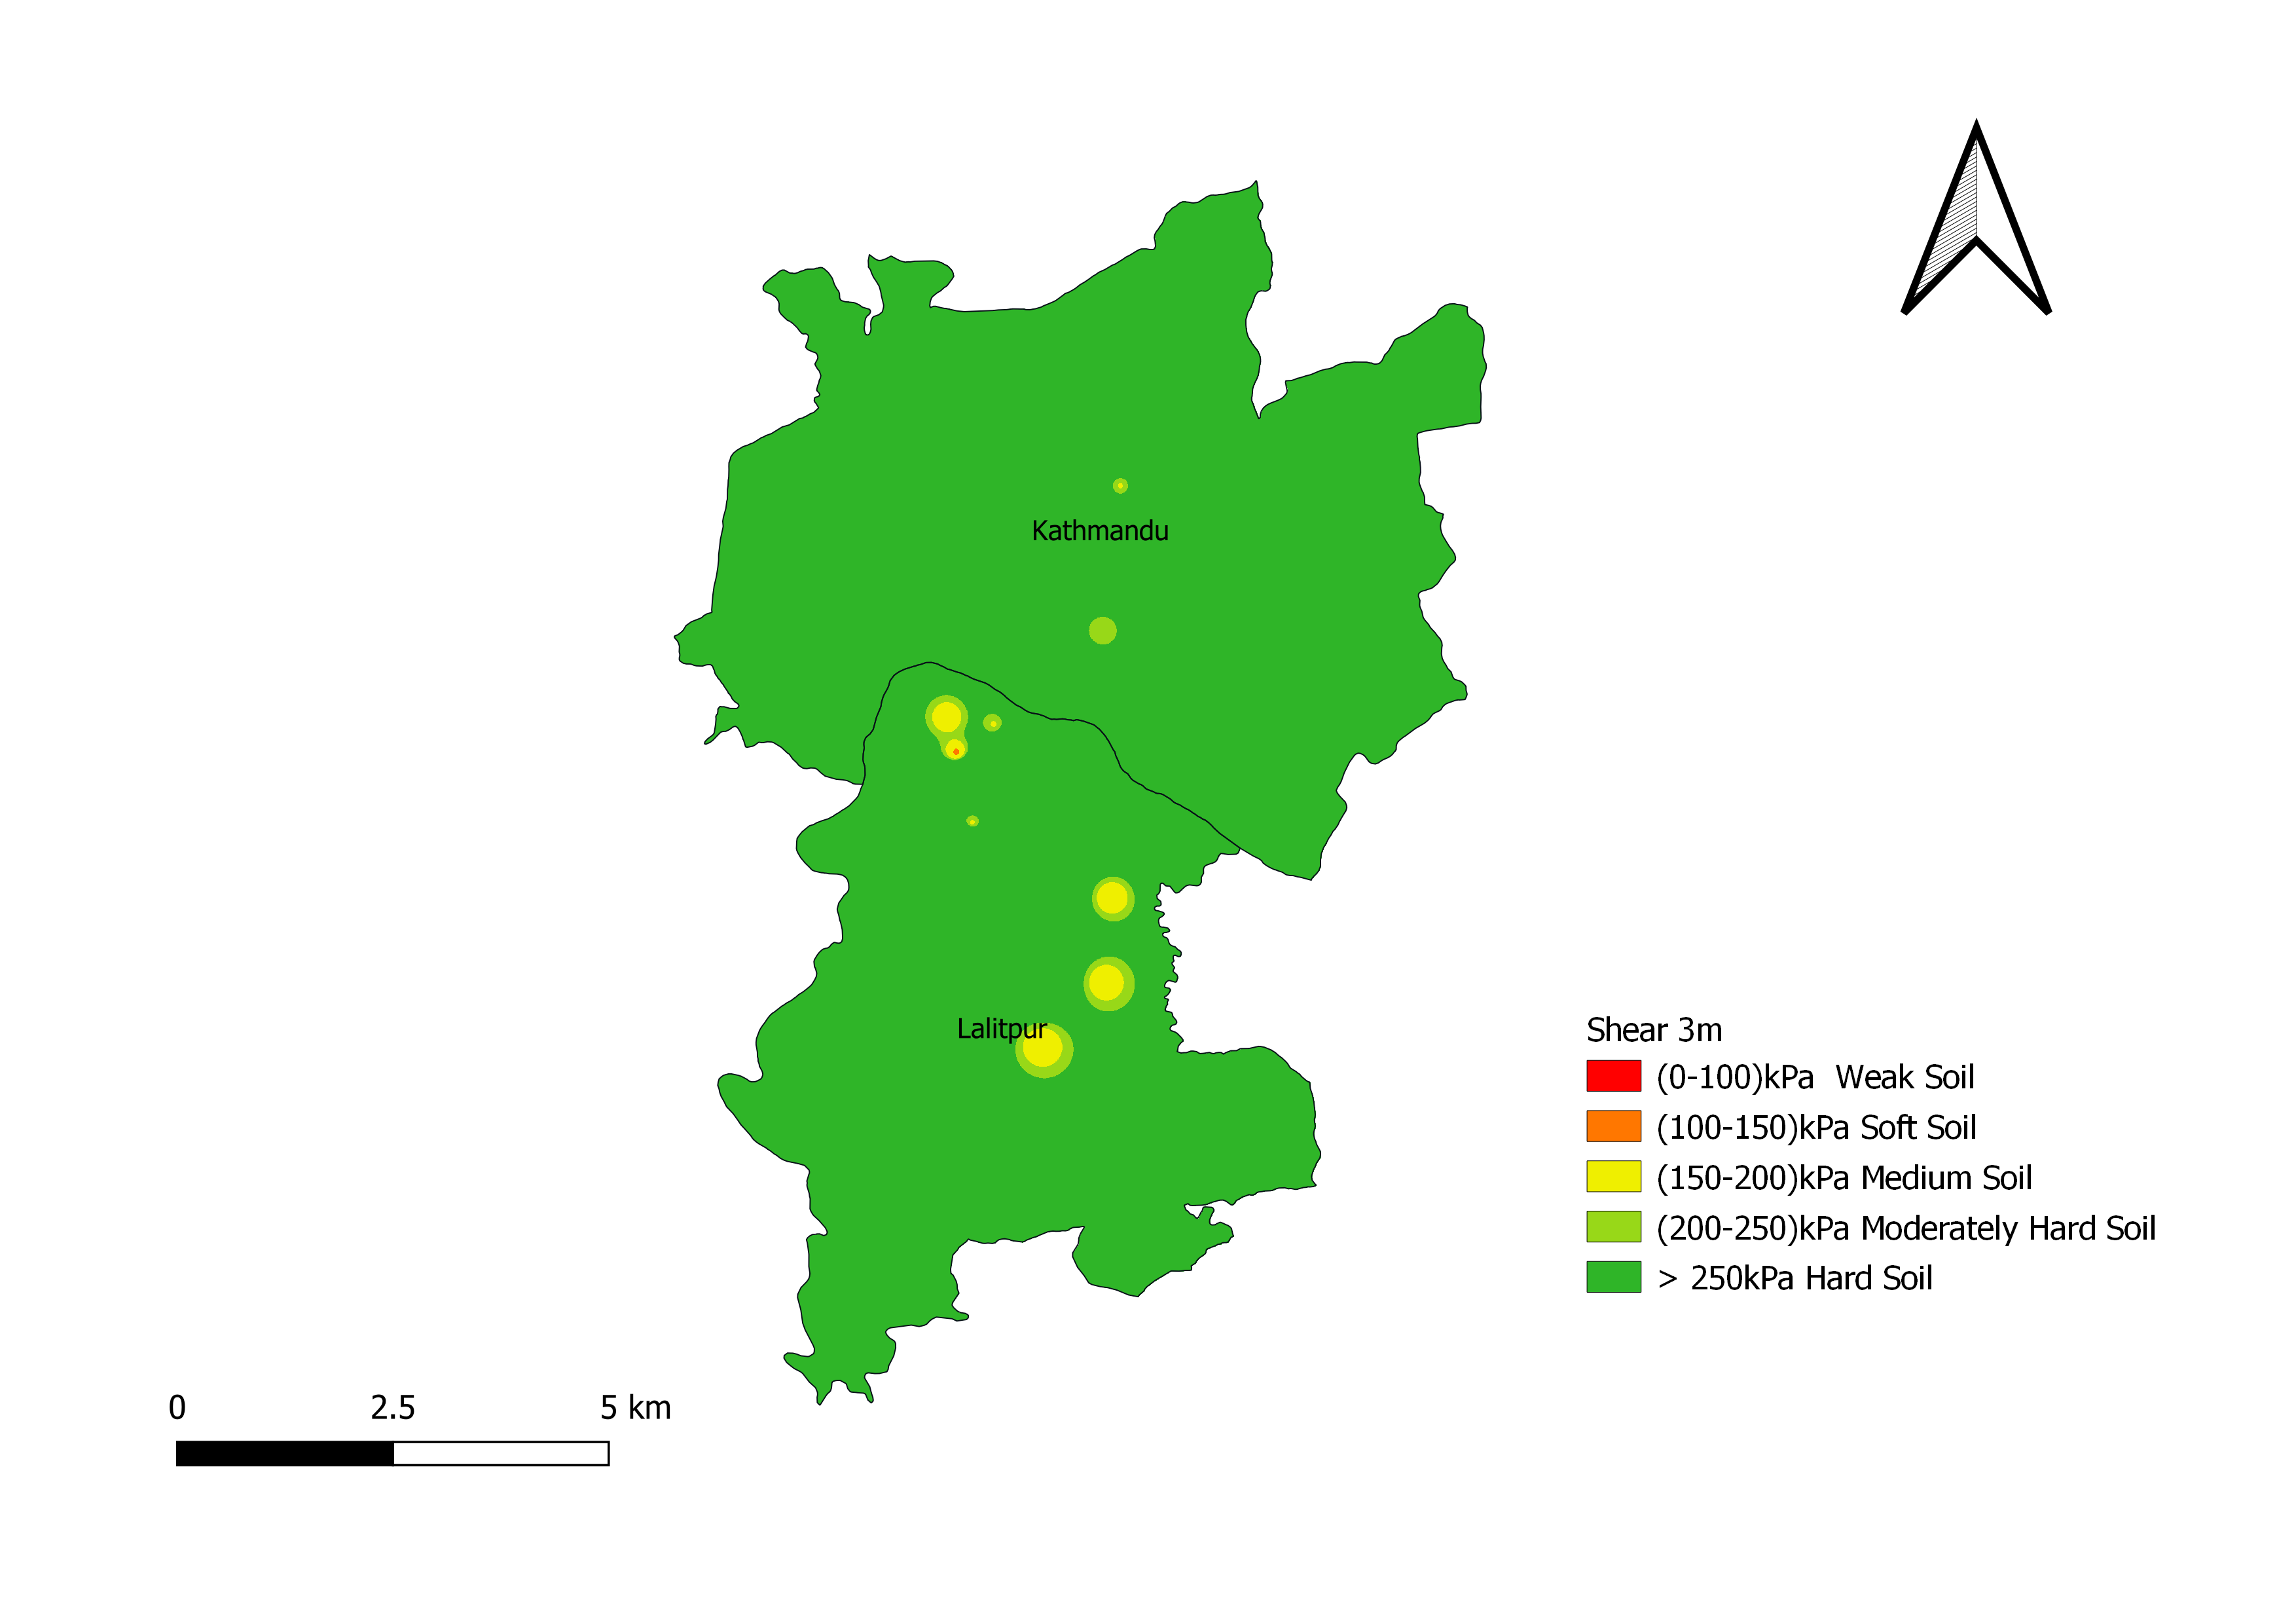
\includegraphics[width=0.8\linewidth, height=0.8\textheight,keepaspectratio]{in/map/Shear_3_0.png}
\caption{BC at 3.0m depth}
\end{figure}
\pagebreak
\end{landscape}

\begin{landscape}
\section{4.5m Bearing Capacity(shear)\index{map}}
\begin{figure}[!hbt]
\centering
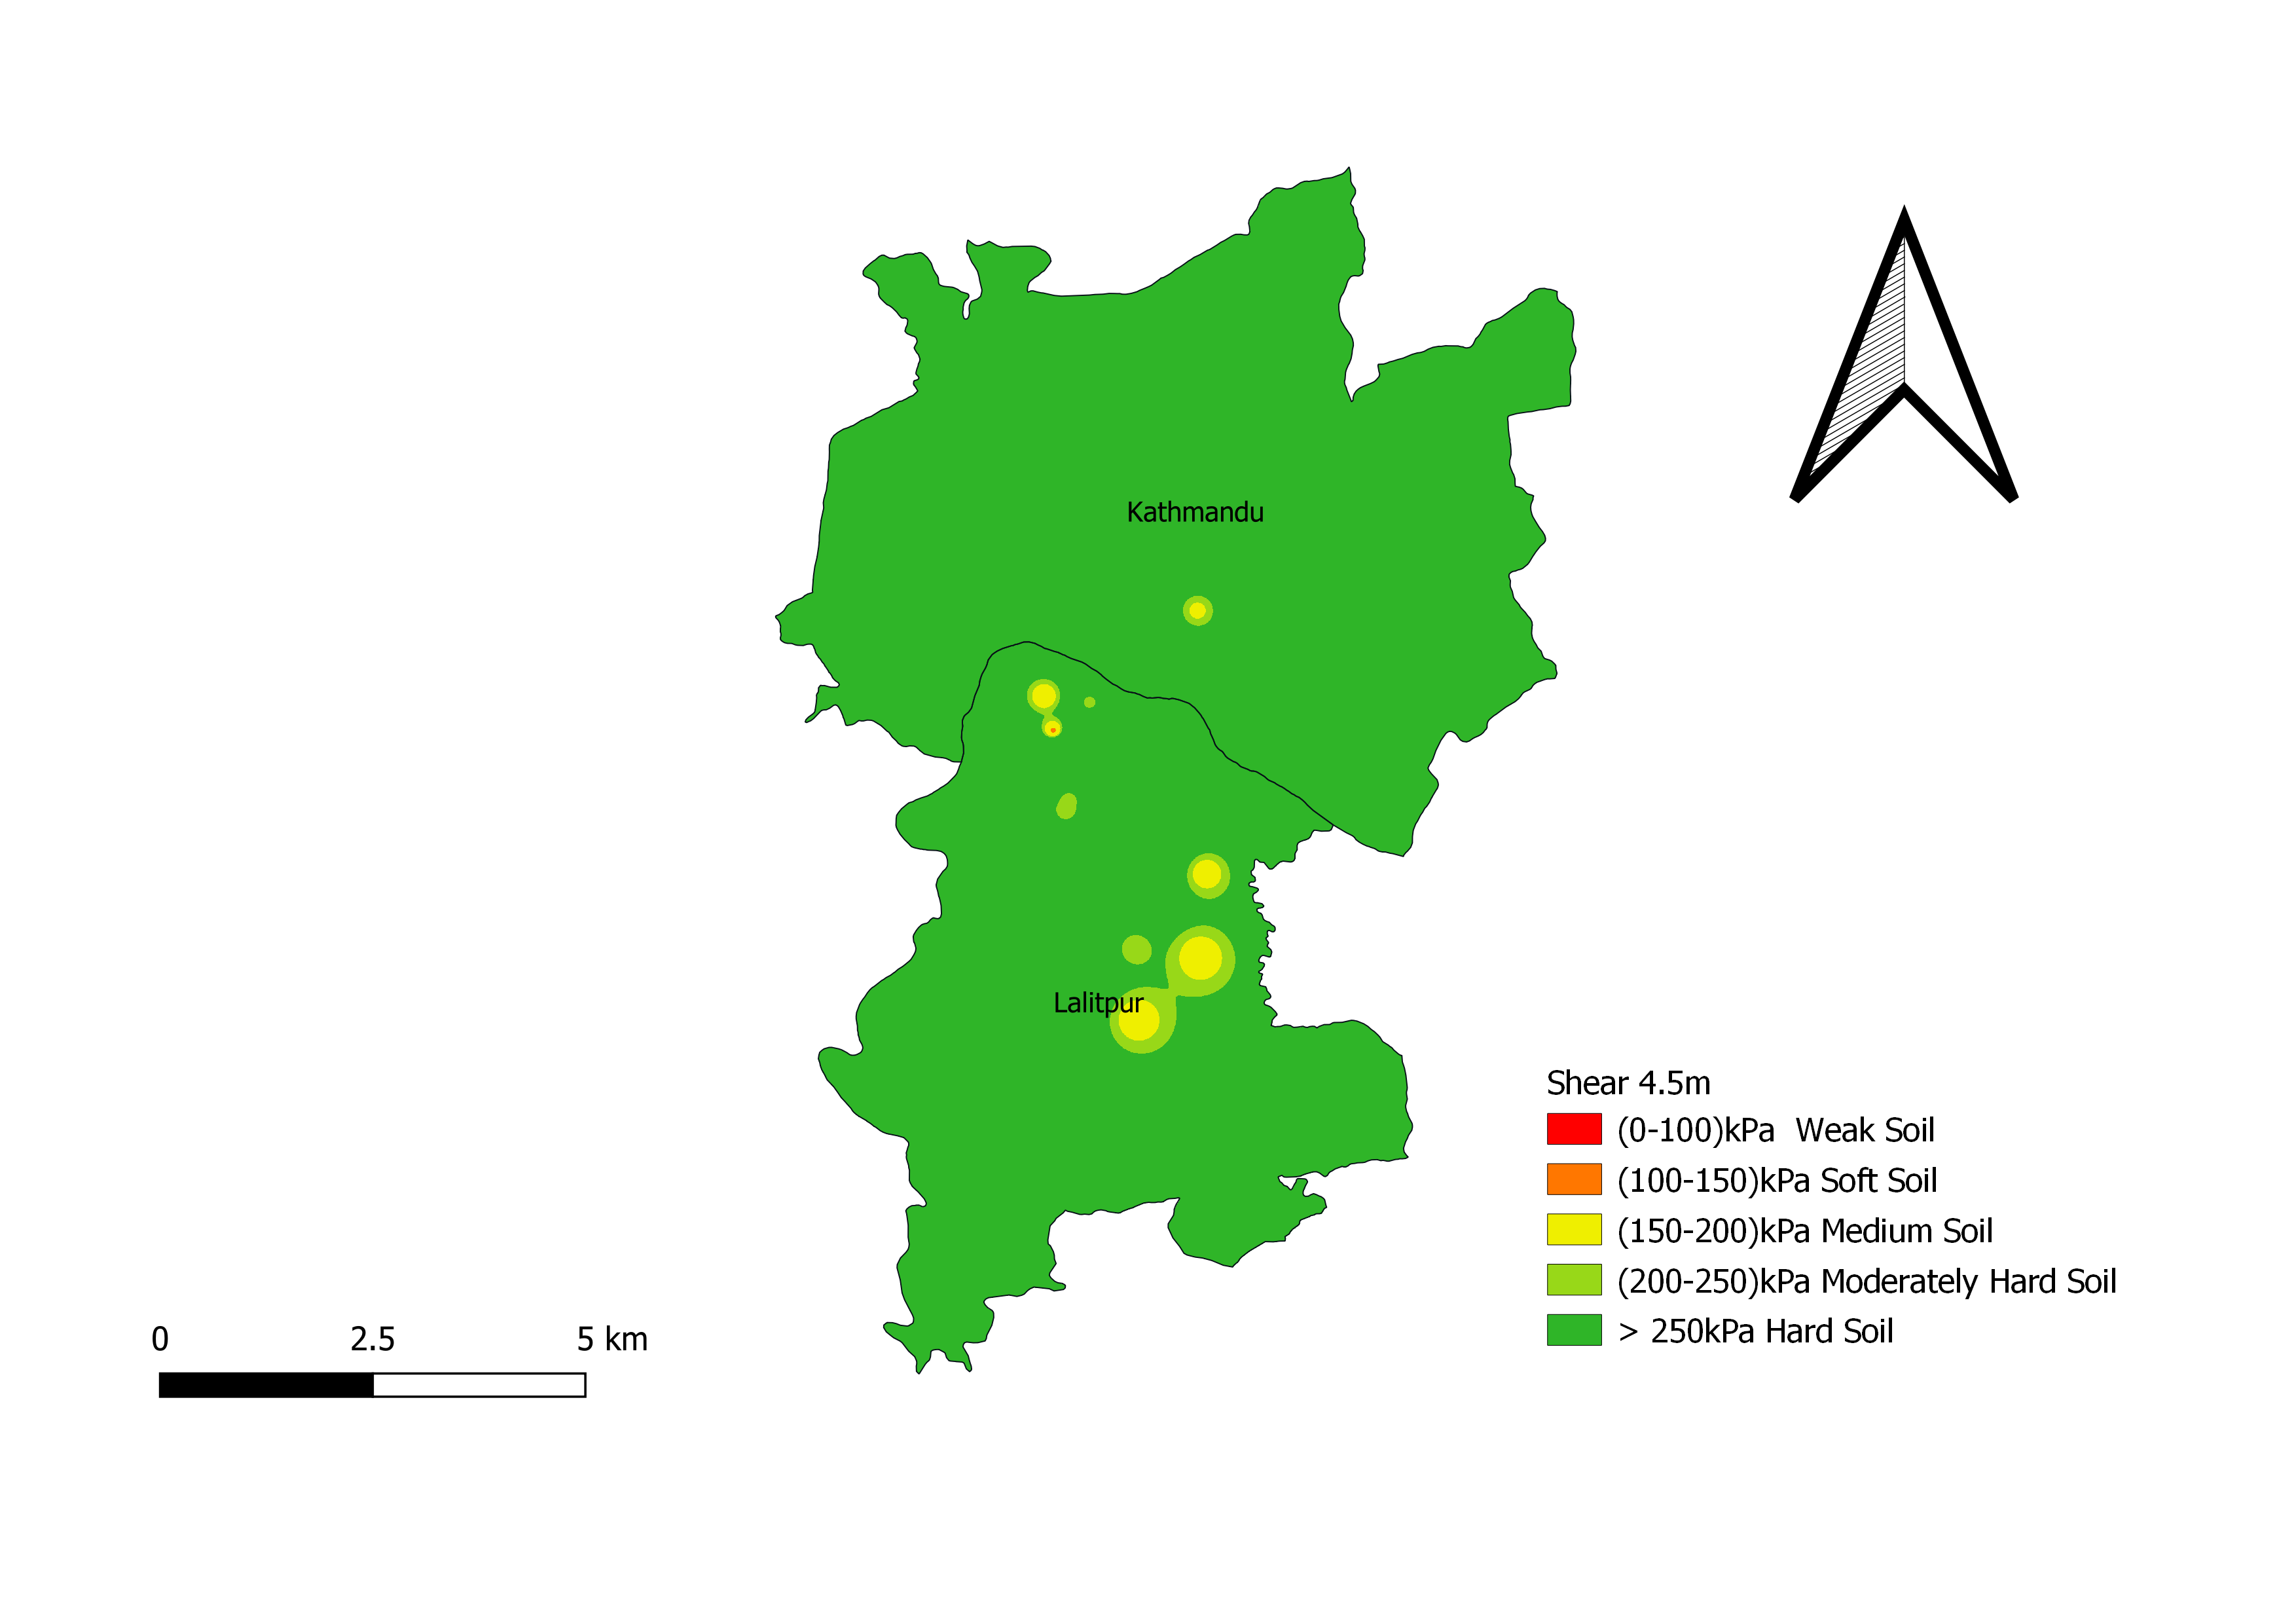
\includegraphics[width=0.8\linewidth, height=0.8\textheight,keepaspectratio]{in/map/Shear_4_5.png}
\caption{BC at 4.5m depth}
\end{figure}
\pagebreak
\end{landscape}

\section{Settlement Strength Table(kPa, for 25mm)}
\begin{table}[!h]
\caption{Settlement Strength Table}
\begin{tabularx}{\textwidth}{ | l | p{0.5\textwidth} | X | X | X | }
\hline
 \textbf{S.N.} & \textbf{Location} & \textbf{1.5m} & \textbf{3.0m} & \textbf{4.5m}\\
\hline
 1 & Thapathali, Kathmandu & 32.327 & 38.642 & 50.943 \\
 2 & Anamnagar, Kathmandu & 178.573 & 98.242 & 71.612 \\
 3 & Bakhundol Lalitpur & 44.627 & 44.584 & 45.737 \\
 4 & Balkumari, Lalitpur & 277.689 & 199.590 & 138.268 \\
 5 & Bansbari, Kathmandu & 143.756 & 135.484 & 150.310 \\
 6 & Bhaisipati, Lalitpur & 310.341 & 303.309 & 200.444 \\
 7 & Gahanapokhari, Kathmandu & 145.774 & 155.979 & 145.323 \\
 8 & Mulpani, Kathamndu  & 65.598 & 120.769 & 182.885 \\
 9 & Itachhe tol, Bhaktapur & 71.789 & 74.786 & 83.443 \\
 10 & Jawalakhel, Lalitpur  & 371.723 & 312.830 & 175.017 \\
 11 & Jawalakhel & 226.421 & 359.938 & 174.803 \\
 12 & Tangal, Kathmandu & 174.929 & 133.731 & 129.194 \\
 13 & Harihar Bhavan, Lalitpur & 43.732 & 41.417 & 39.361 \\
 14 & Kuleswore, Kathmandu & 91.046 & 66.566 & 50.069 \\
 15 & Lainchour, Kathmandu & 182.240 & 245.151 & 236.805 \\
 16 & Tahachal, Kathmandu & 43.164 & 60.422 & 72.989 \\
 17 & Satdobato, Lalitpur & 510.209 & 252.241 & 144.841 \\
 18 & Naxal, Nagpokhari Kathmandu  & 73.785 & 85.657 & 108.810 \\
 19 & Mandikatar, Kathmandu  & 248.511 & 248.768 & 168.528 \\
 20 & Mandikhatar, Kathmandu  & 127.783 & 266.774 & 281.543 \\
 21 & Lainchaur, Kathmandu  & 174.929 & 181.025 & 188.245 \\
 22 & Kupondole, Lalitpur & 248.511 & 319.444 & 341.663 \\
 23 & Kupondole, Lalitpur & 143.756 & 104.626 & 97.679 \\
 24 & Khumaltar, Lalitpur & 133.930 & 60.043 & 48.454 \\
 25 & Khumaltar, Lalitpur  & 109.923 & 101.519 & 83.482 \\
 26 & Kalopul, Pumori, Kathmandu & 119.431 & 112.012 & 101.643 \\
 27 & Gwarkho, Lalitpur & 76.146 & 76.876 & 62.440 \\
 28 & Kumaripati, Lalitpur & 606.172 & 523.712 & 466.218 \\
 29 & Kupandole, Lalitpur & 53.935 & 50.015 & 49.253 \\
 30 & Thapathali & 105.779 & 85.681 & 77.141 \\
 31 & Kirtipur, Kathmandu & 103.824 & 89.948 & 65.702 \\
\hline
\multicolumn{2}{|X|}{\mbox{Mean($\overline{x}$)}} & 142.206 & 147.536 & 118.102 \\
\multicolumn{2}{|X|}{\mbox{Standard deviation($\sigma$)}} & 85.117 & 94.886 & 62.637 \\
\multicolumn{2}{|X|}{\mbox{Minimum($x_{min}$)}} & 32.327 & 38.642 & 39.361 \\
\multicolumn{2}{|X|}{\mbox{Maximum($x_{max}$)}} & 371.723 & 359.938 & 281.543 \\
\hline
\end{tabularx}

\end{table}
\pagebreak

\begin{landscape}
\section{1.5m Bearing Capacity(settlement)\index{map}}
\begin{figure}[!hbt]
\centering
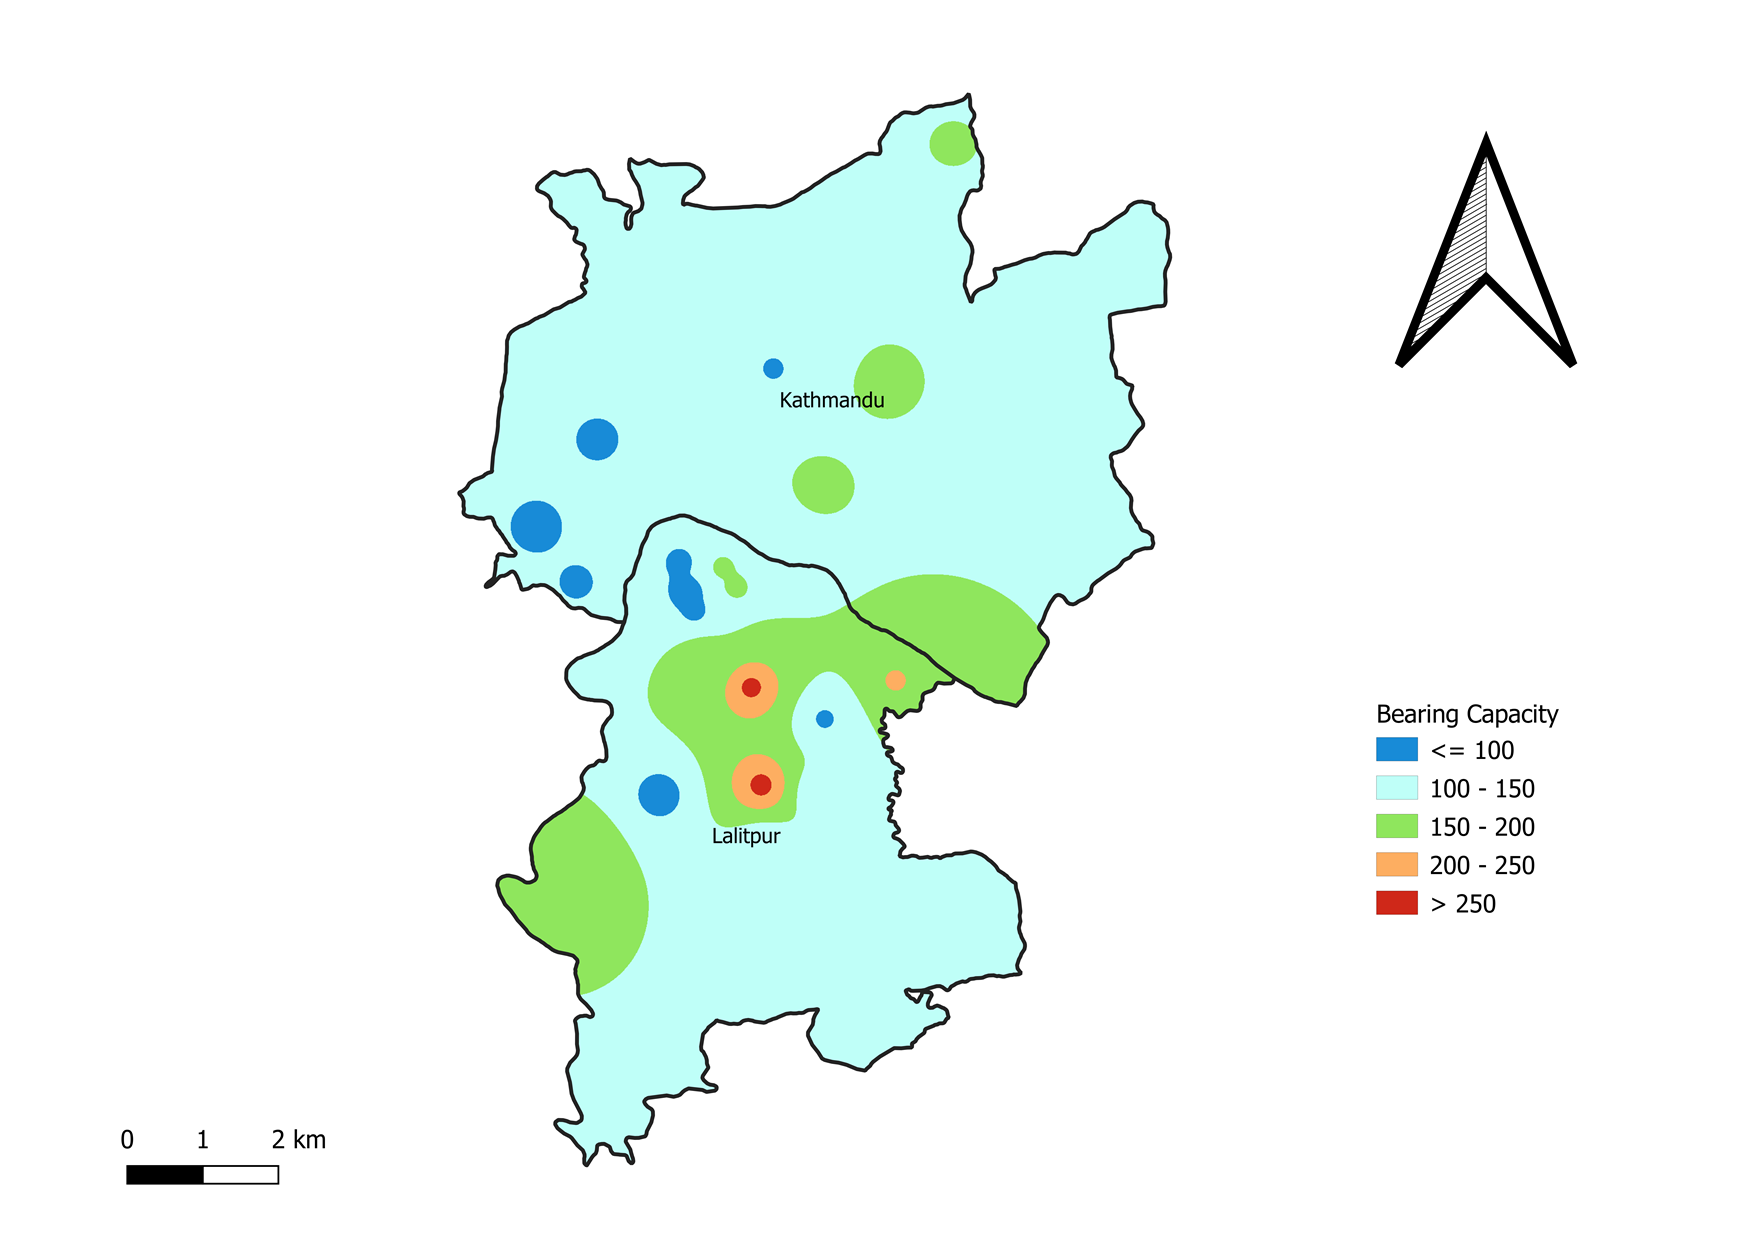
\includegraphics[width=0.8\linewidth, height=0.8\textheight,keepaspectratio]{in/map/Deflection_1_5.png}
\caption{BC at 1.5m depth}
\end{figure}
\pagebreak
\end{landscape}

\begin{landscape}
\section{3.0m Bearing Capacity(settlement)\index{map}}
\begin{figure}[!hbt]
\centering
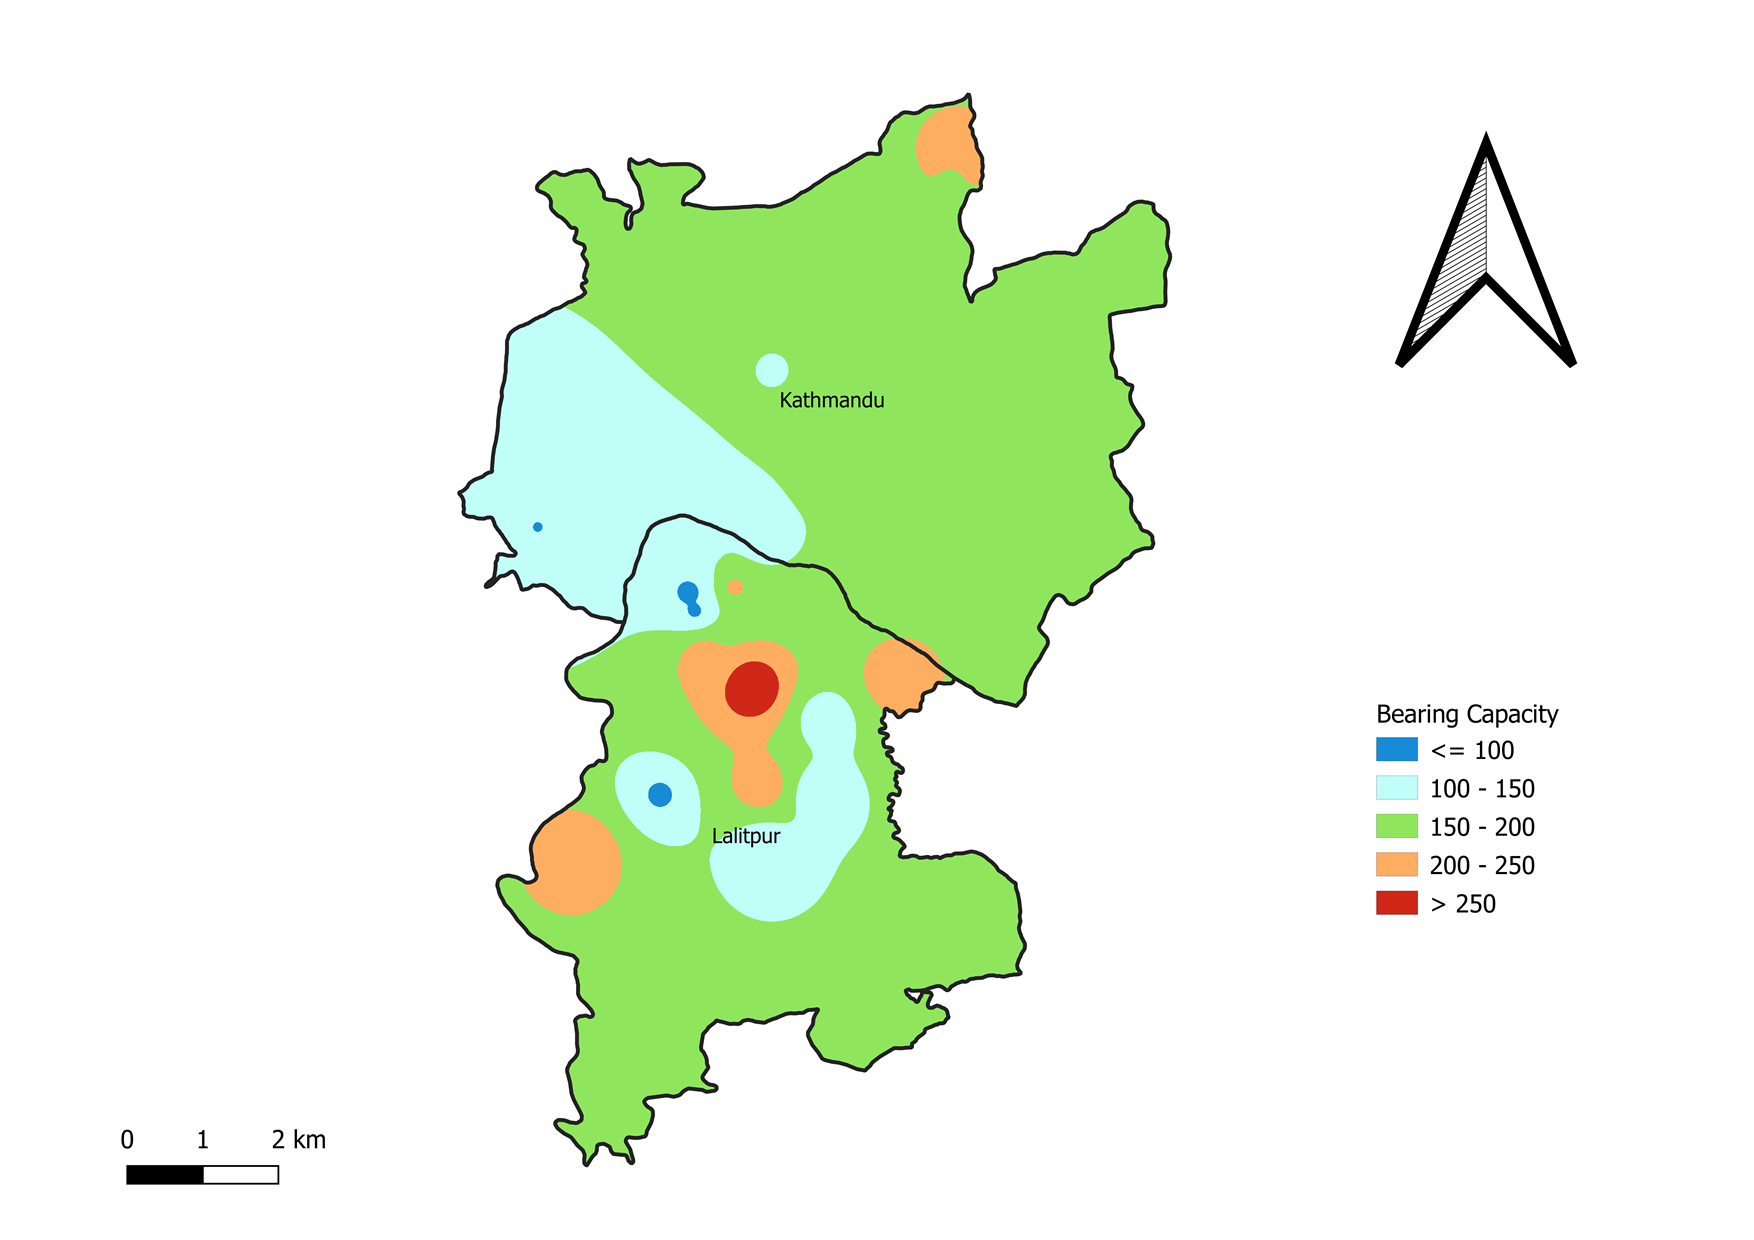
\includegraphics[width=0.8\linewidth, height=0.8\textheight,keepaspectratio]{in/map/Deflection_3_0.png}
\caption{BC at 3.0m depth}
\end{figure}
\pagebreak
\end{landscape}

\begin{landscape}
\section{4.5m Bearing Capacity(settlement)\index{map}}
\begin{figure}[!hbt]
\centering
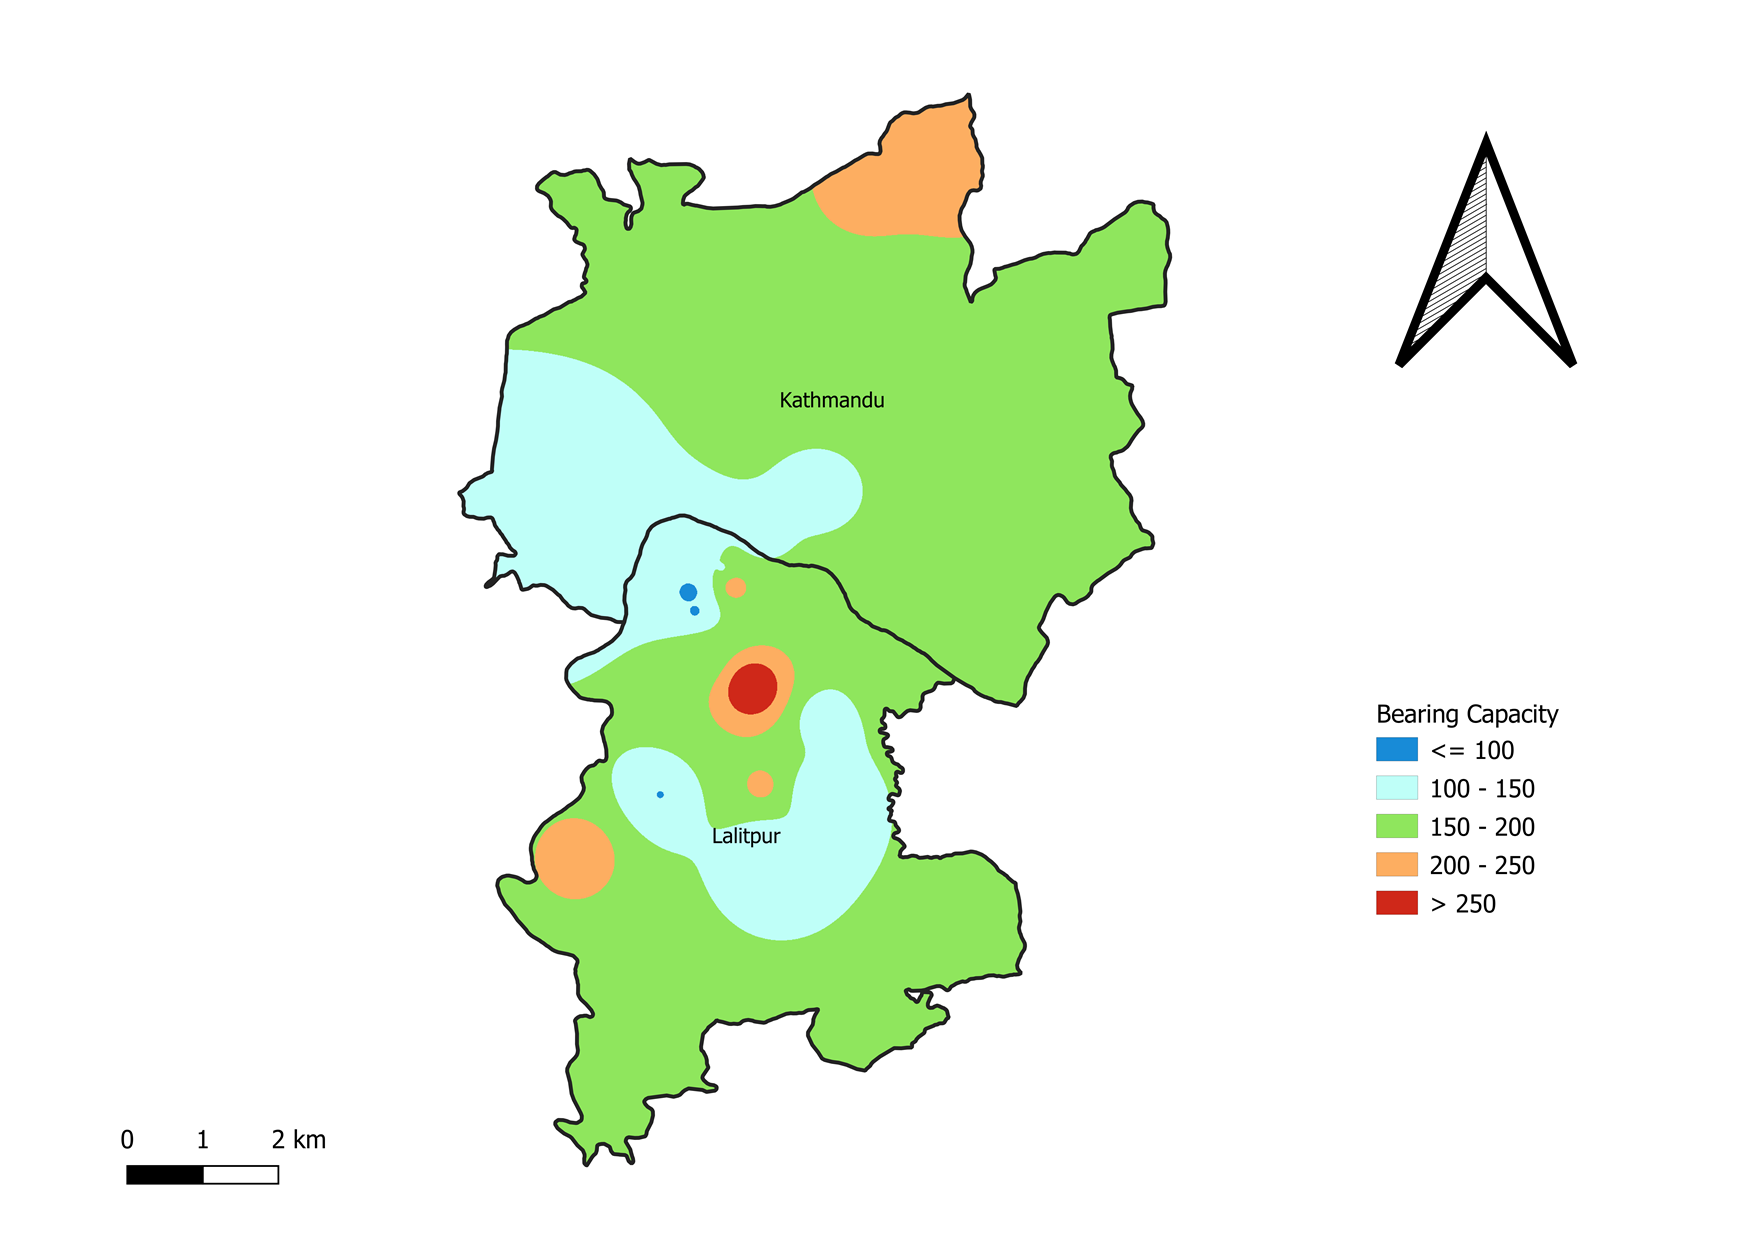
\includegraphics[width=0.8\linewidth, height=0.8\textheight,keepaspectratio]{in/map/Deflection_4_5.png}
\caption{BC at 3.0m depth}
\end{figure}
\pagebreak
\end{landscape}

\begin{landscape}
\section{Relation of depth vs Bearing Capacity}
\begin{figure}[!hbt]
\centering
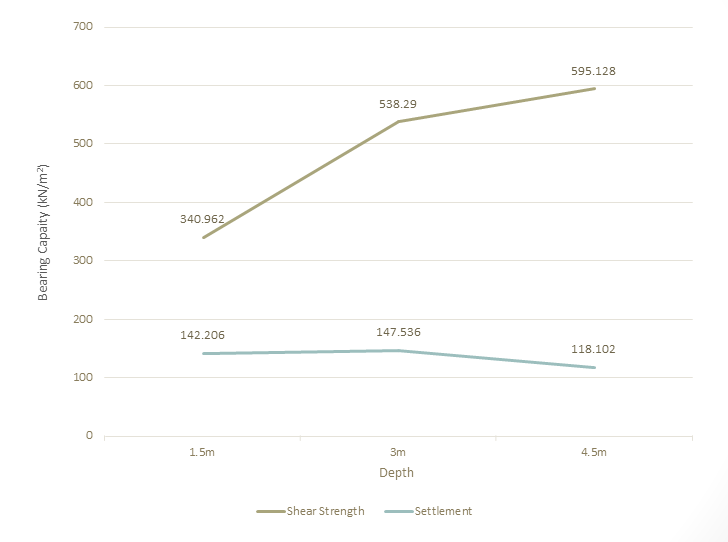
\includegraphics[width=0.8\linewidth, height=0.8\textheight,keepaspectratio]{images/main/d_vs_bc.png}
\caption{Relation of depth vs Bearing Capacity}
\end{figure}
\pagebreak
\end{landscape}

\section{Net Allowable Strength Table(kPa, for 25mm)}
\begin{table}[!h]
\caption{Net Allowable Strength Table}
\begin{tabularx}{\textwidth}{ | l | p{0.5\textwidth} | X | X | X | }
\hline
 \textbf{S.N.} & \textbf{Location} & \textbf{1.5m} & \textbf{3.0m} & \textbf{4.5m}\\
\hline
 1 & Thapathali, Kathmandu & 32.327 & 38.642 & 50.943 \\
 2 & Anamnagar, Kathmandu & 178.573 & 98.242 & 71.612 \\
 3 & Bakhundol Lalitpur & 44.627 & 44.584 & 45.737 \\
 4 & Balkumari, Lalitpur & 277.689 & 199.590 & 138.268 \\
 5 & Bansbari, Kathmandu & 143.756 & 135.484 & 150.310 \\
 6 & Bhaisipati, Lalitpur & 310.341 & 303.309 & 200.444 \\
 7 & Gahanapokhari, Kathmandu & 145.774 & 155.979 & 145.323 \\
 8 & Mulpani, Kathamndu  & 65.598 & 120.769 & 182.885 \\
 9 & Itachhe tol, Bhaktapur & 71.789 & 74.786 & 83.443 \\
 10 & Jawalakhel, Lalitpur  & 295.379 & 312.830 & 175.017 \\
 11 & Jawalakhel & 154.538 & 188.042 & 174.803 \\
 12 & Tangal, Kathmandu & 174.929 & 133.731 & 129.194 \\
 13 & Harihar Bhavan, Lalitpur & 43.732 & 41.417 & 39.361 \\
 14 & Kuleswore, Kathmandu & 91.046 & 66.566 & 50.069 \\
 15 & Lainchour, Kathmandu & 182.240 & 245.151 & 236.805 \\
 16 & Tahachal, Kathmandu & 43.164 & 60.422 & 72.989 \\
 17 & Satdobato, Lalitpur & 510.209 & 252.241 & 144.841 \\
 18 & Naxal, Nagpokhari Kathmandu  & 73.785 & 85.657 & 108.810 \\
 19 & Mandikatar, Kathmandu  & 216.255 & 248.768 & 168.528 \\
 20 & Mandikhatar, Kathmandu  & 127.783 & 266.774 & 281.543 \\
 21 & Lainchaur, Kathmandu  & 174.929 & 181.025 & 188.245 \\
 22 & Kupondole, Lalitpur & 197.198 & 319.444 & 341.663 \\
 23 & Kupondole, Lalitpur & 143.756 & 104.626 & 97.679 \\
 24 & Khumaltar, Lalitpur & 130.857 & 60.043 & 48.454 \\
 25 & Khumaltar, Lalitpur  & 109.923 & 101.519 & 83.482 \\
 26 & Kalopul, Pumori, Kathmandu & 119.431 & 112.012 & 101.643 \\
 27 & Gwarkho, Lalitpur & 76.146 & 76.876 & 62.440 \\
 28 & Kumaripati, Lalitpur & 606.172 & 523.712 & 466.218 \\
 29 & Kupandole, Lalitpur & 53.935 & 50.015 & 49.253 \\
 30 & Thapathali & 105.779 & 85.681 & 77.141 \\
 31 & Kirtipur, Kathmandu & 103.824 & 89.948 & 65.702 \\
\hline
\multicolumn{2}{|X|}{\mbox{Mean($\overline{x}$)}} & 134.107 & 141.806 & 118.102 \\
\multicolumn{2}{|X|}{\mbox{Standard deviation($\sigma$)}} & 73.815 & 86.726 & 62.637 \\
\multicolumn{2}{|X|}{\mbox{Minimum($x_{min}$)}} & 32.327 & 38.642 & 39.361 \\
\multicolumn{2}{|X|}{\mbox{Maximum($x_{max}$)}} & 310.341 & 319.444 & 281.543 \\
\hline
\end{tabularx}

\end{table}
\pagebreak

\begin{landscape}
\section{1.5m Bearing Capacity(Net Allowable)\index{map}}
\begin{figure}[!hbt]
\centering
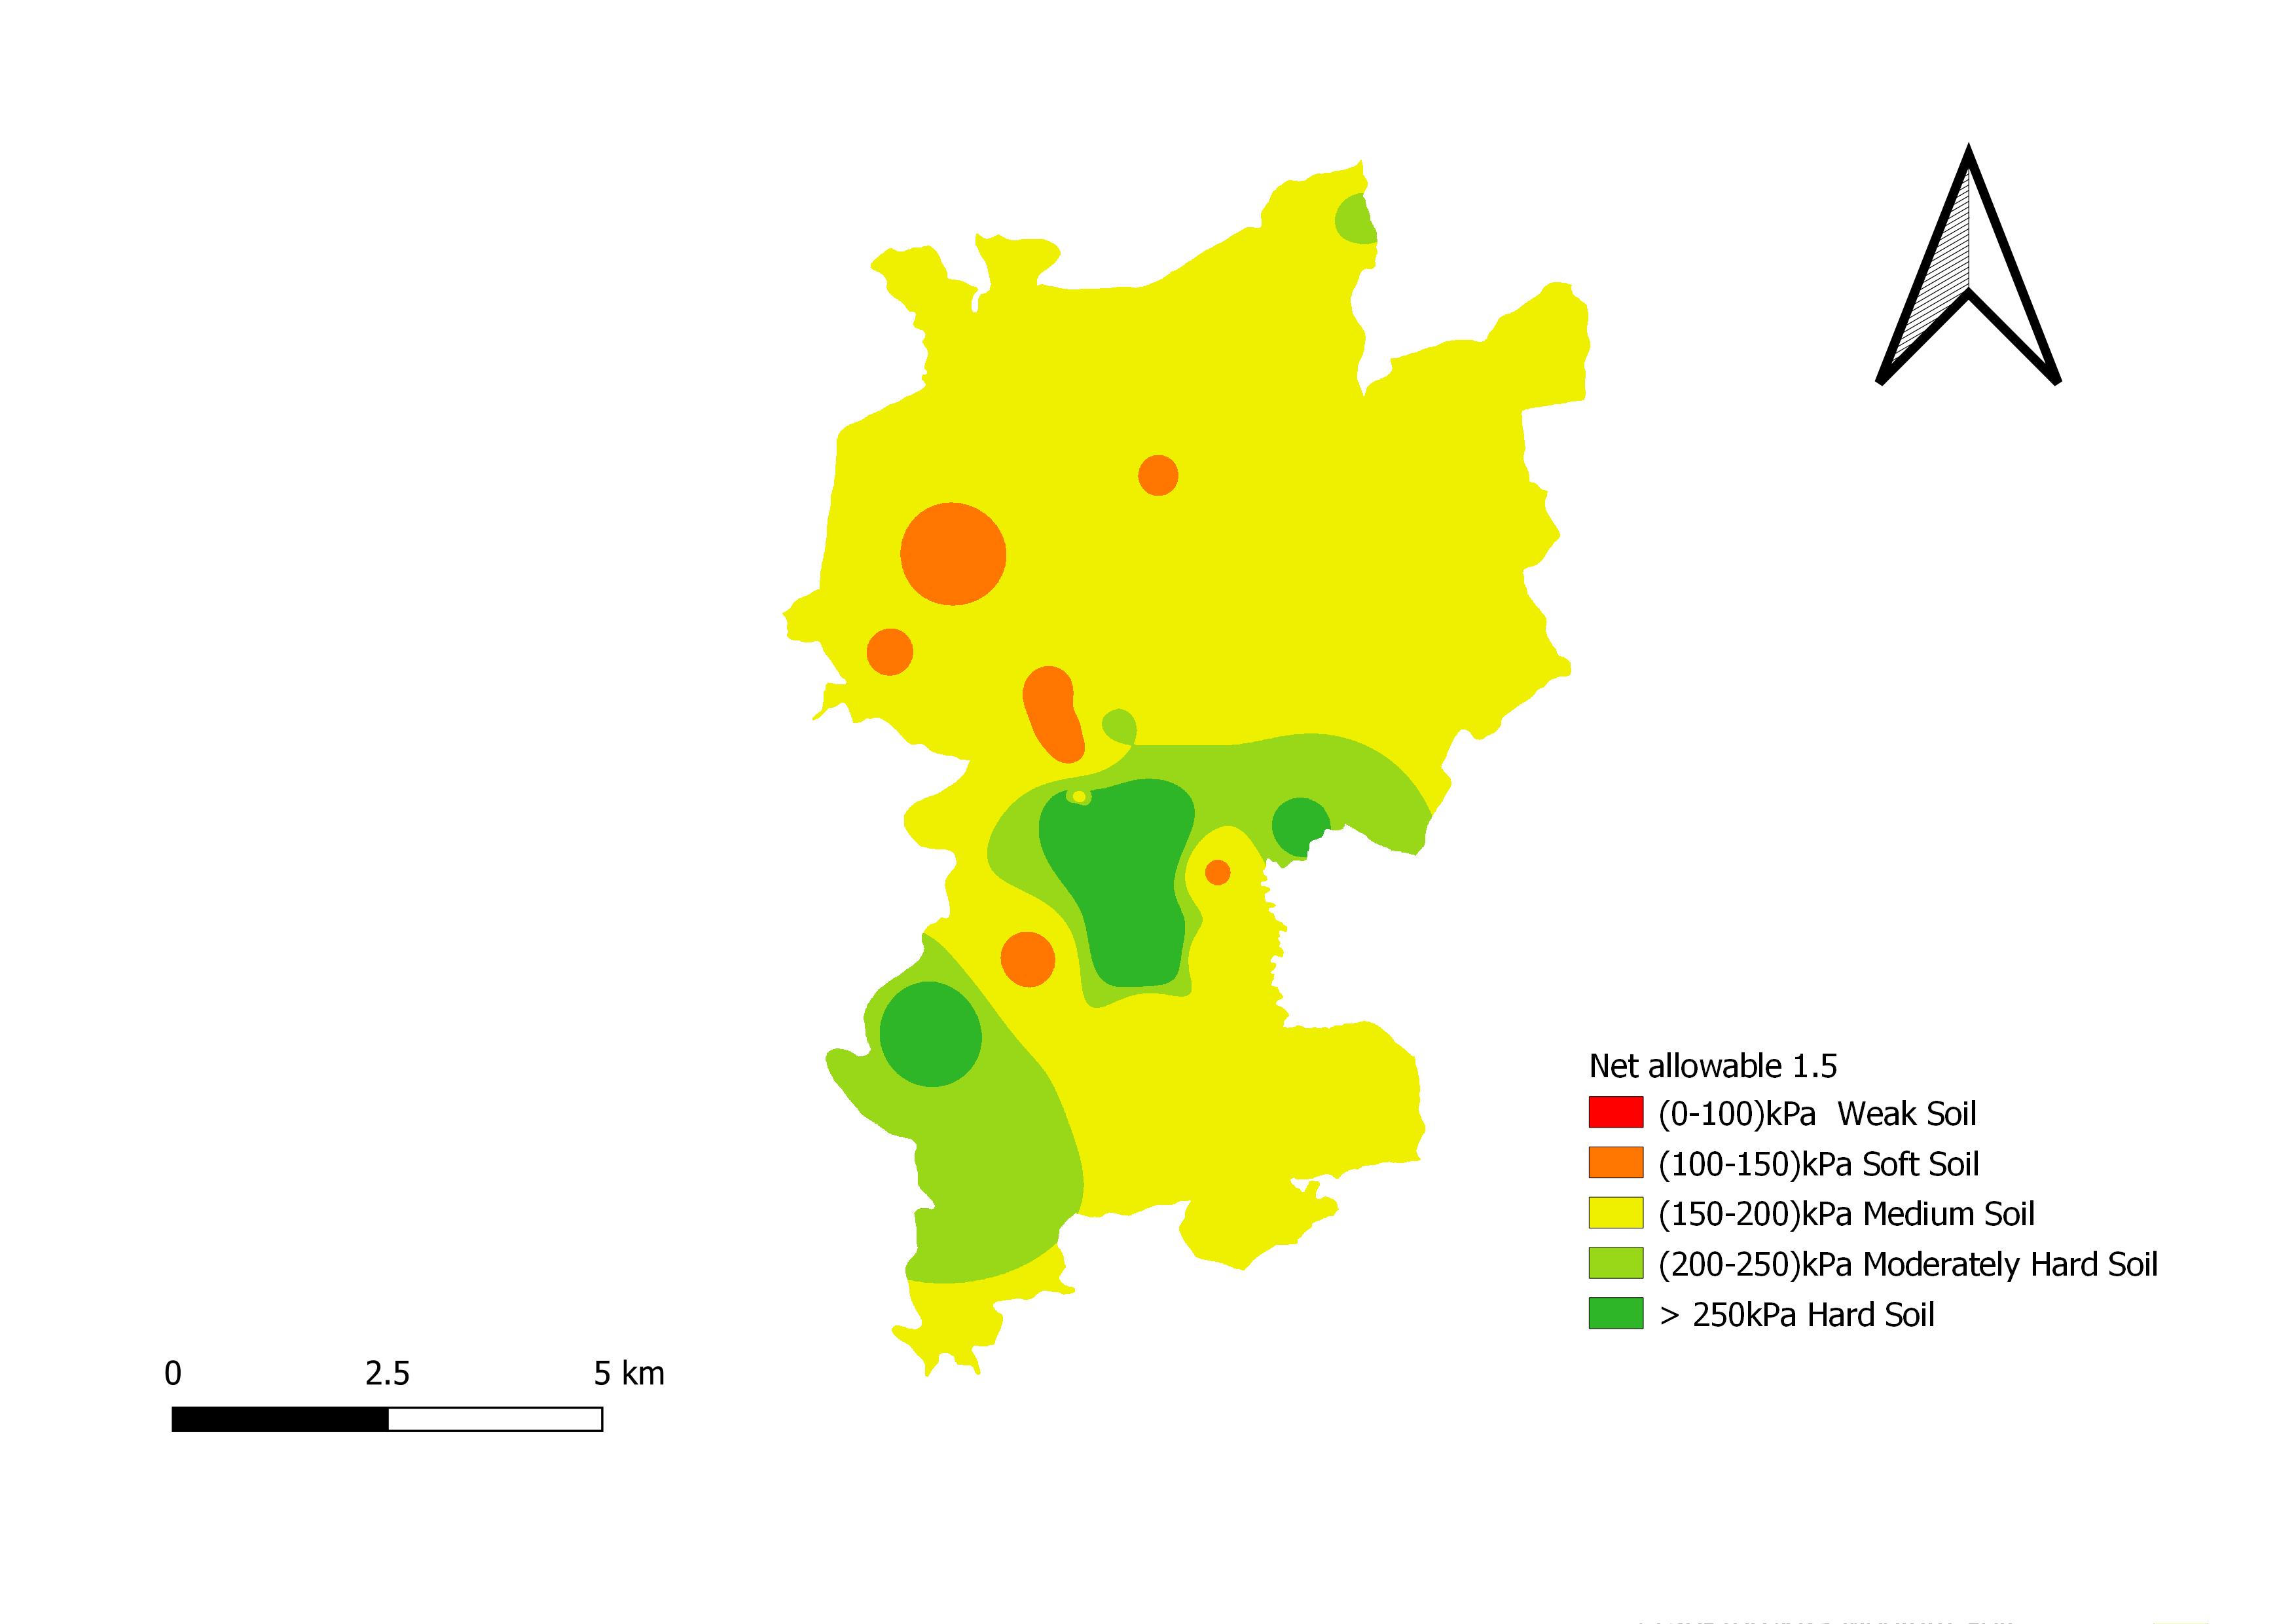
\includegraphics[width=0.8\linewidth, height=0.8\textheight,keepaspectratio]{in/map/na_1_5.png}
\caption{BC at 1.5m depth}
\end{figure}
\pagebreak
\end{landscape}

\begin{landscape}
\section{3.0m Bearing Capacity(Net Allowable)\index{map}}
\begin{figure}[!hbt]
\centering
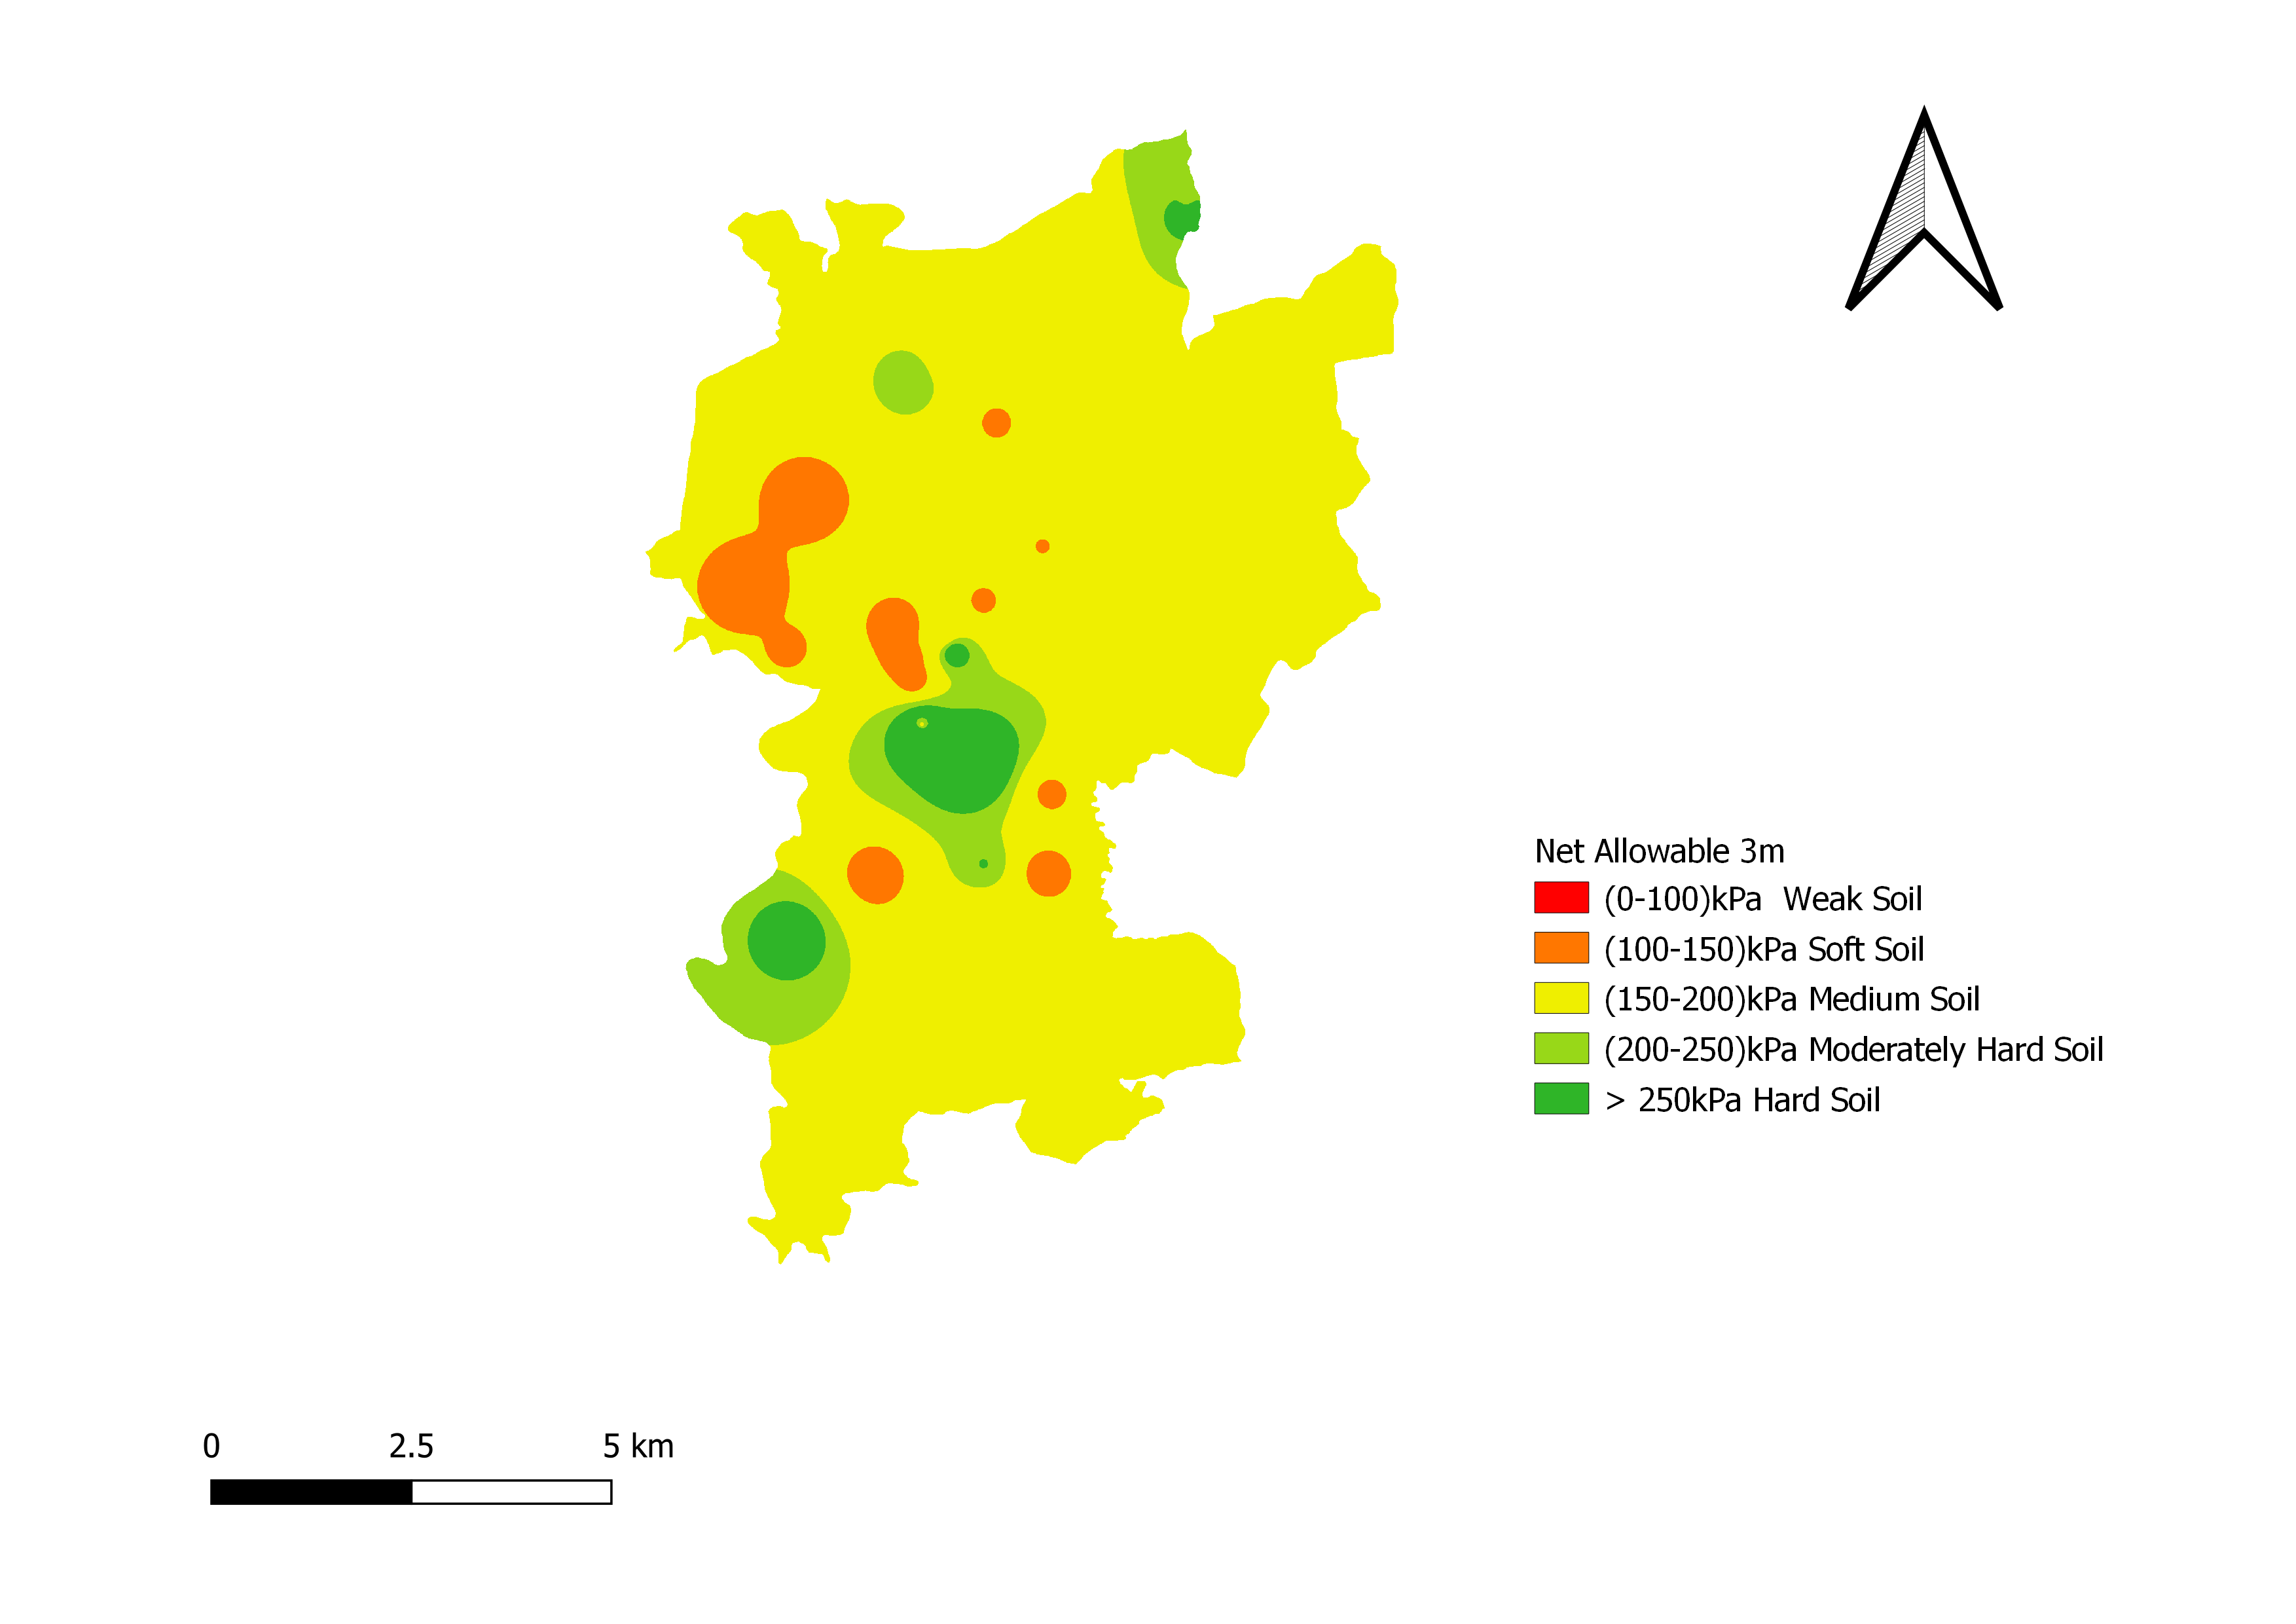
\includegraphics[width=0.8\linewidth, height=0.8\textheight,keepaspectratio]{in/map/na_3_0.png}
\caption{BC at 3.0m depth}
\end{figure}
\pagebreak
\end{landscape}

\begin{landscape}
\section{4.5m Bearing Capacity(Net Allowable)\index{map}}
\begin{figure}[!hbt]
\centering
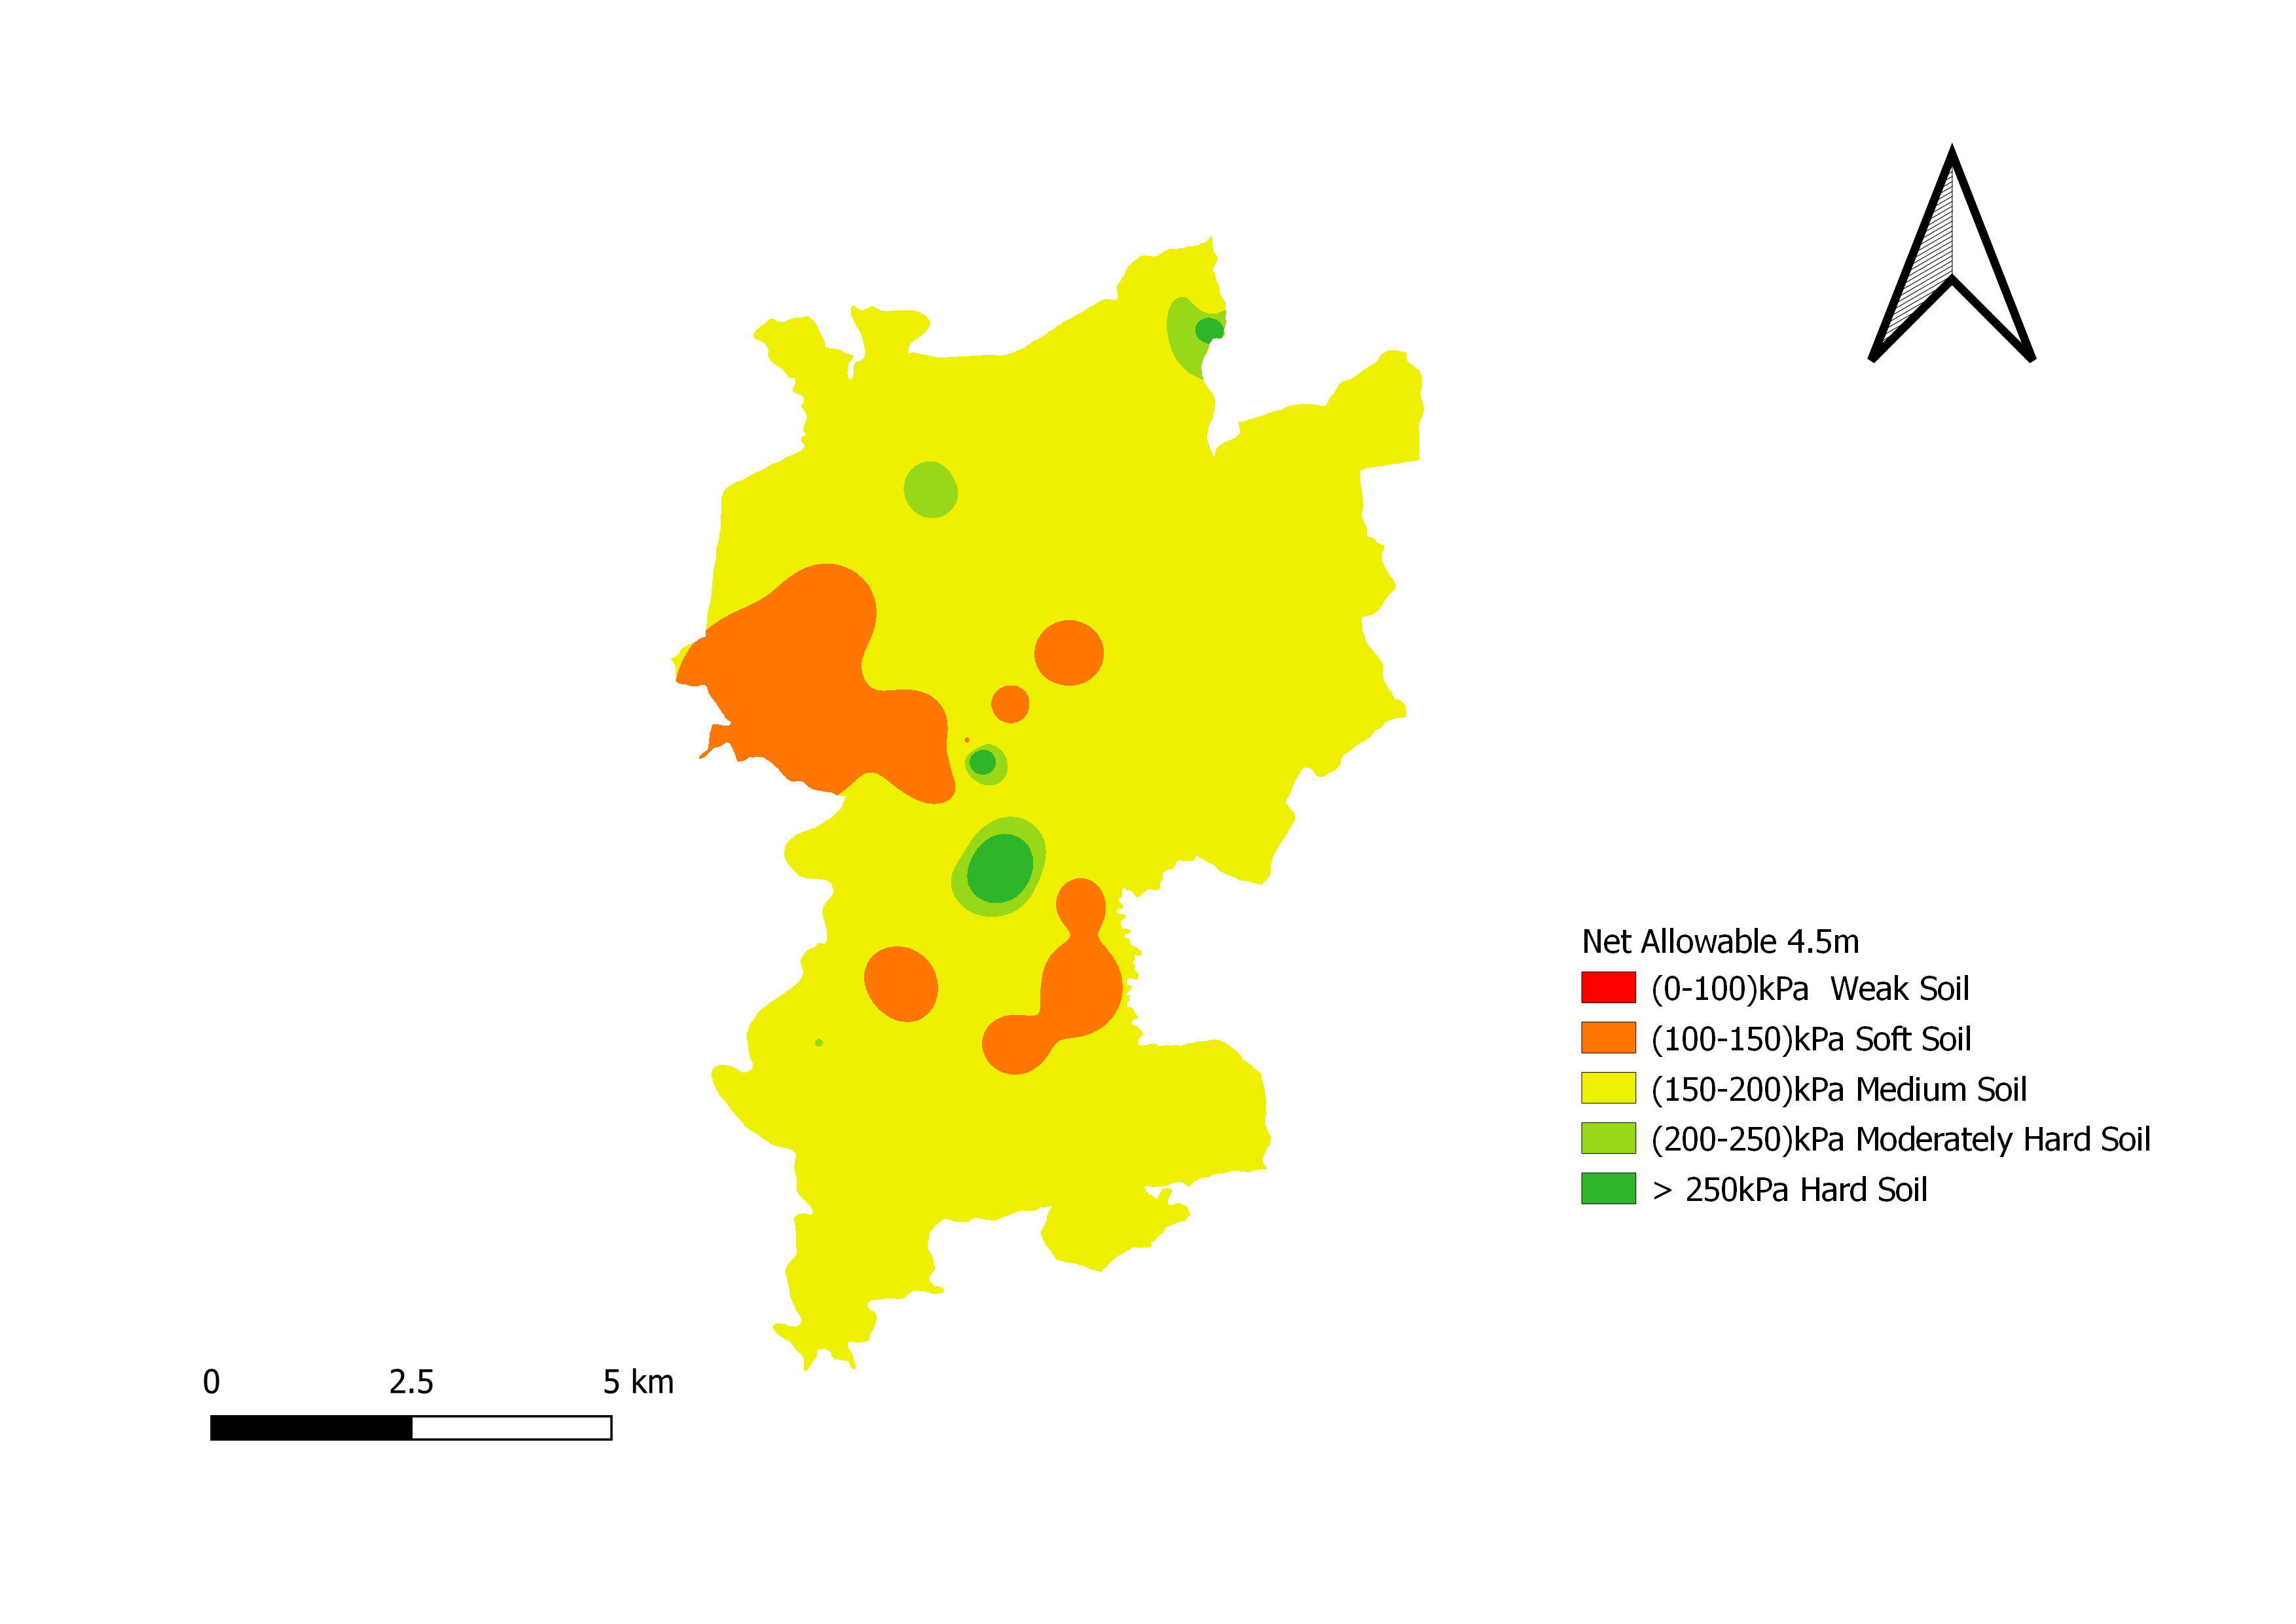
\includegraphics[width=0.8\linewidth, height=0.8\textheight,keepaspectratio]{in/map/na_4_5.png}
\caption{BC at 4.5m depth}
\end{figure}
\pagebreak
\end{landscape}

\section{Liquefaction(LPI) Table}
\begin{table}[!h]
\caption{Liquefaction(LPI) Table}
\begin{tabularx}{\textwidth}{ | l | p{0.5\textwidth} | X | }
\hline
 \textbf{S.N.} & \textbf{Location} & \textbf{LPI}\\
\hline
 1 & Thapathali, Kathmandu & 26.184 \\
 2 & Anamnagar, Kathmandu & 18.597 \\
 3 & Bakhundol Lalitpur & 6.858 \\
 4 & Balkumari, Lalitpur & 16.423 \\
 5 & Bansbari, Kathmandu & 1.518 \\
 6 & Bhaisipati, Lalitpur & 0.045 \\
 7 & Gahanapokhari, Kathmandu & 0.670 \\
 8 & Mulpani, Kathamndu  & 1.325 \\
 9 & Itachhe tol, Bhaktapur & 0.479 \\
 10 & Jawalakhel, Lalitpur  & 0.743 \\
 11 & Jawalakhel & 12.442 \\
 12 & Tangal, Kathmandu & 4.132 \\
 13 & Harihar Bhavan, Lalitpur & 31.190 \\
 14 & Kuleswore, Kathmandu & 17.653 \\
 15 & Lainchour, Kathmandu & 1.319 \\
 16 & Tahachal, Kathmandu & 50.302 \\
 17 & Satdobato, Lalitpur & 0.383 \\
 18 & Naxal, Nagpokhari Kathmandu  & 1.661 \\
 19 & Mandikatar, Kathmandu  & 1.028 \\
 20 & Mandikhatar, Kathmandu  & 2.204 \\
 21 & Lainchaur, Kathmandu  & 4.616 \\
 22 & Kupondole, Lalitpur & 2.649 \\
 23 & Kupondole, Lalitpur & 10.705 \\
 24 & Khumaltar, Lalitpur & 16.796 \\
 25 & Khumaltar, Lalitpur  & 11.200 \\
 26 & Kalopul, Pumori, Kathmandu & 6.137 \\
 27 & Gwarkho, Lalitpur & 19.032 \\
 28 & Kumaripati, Lalitpur & 0.000 \\
 29 & Kupandole, Lalitpur & 20.590 \\
 30 & Thapathali & 4.920 \\
 31 & Kirtipur, Kathmandu & 8.512 \\
\hline
\multicolumn{2}{|X|}{\mbox{Mean($\overline{x}$)}} & 8.334  \\
\multicolumn{2}{|X|}{\mbox{Standard deviation($\sigma$)}} & 8.579 \\
\multicolumn{2}{|X|}{\mbox{Minimum($x_{min}$)}} & 0.000 \\
\multicolumn{2}{|X|}{\mbox{Maximum($x_{max}$)}} & 31.190 \\
\hline
\end{tabularx}

\end{table}
\pagebreak

\begin{landscape}
\section{LPI\index{map}}
\begin{figure}[!h]
\centering
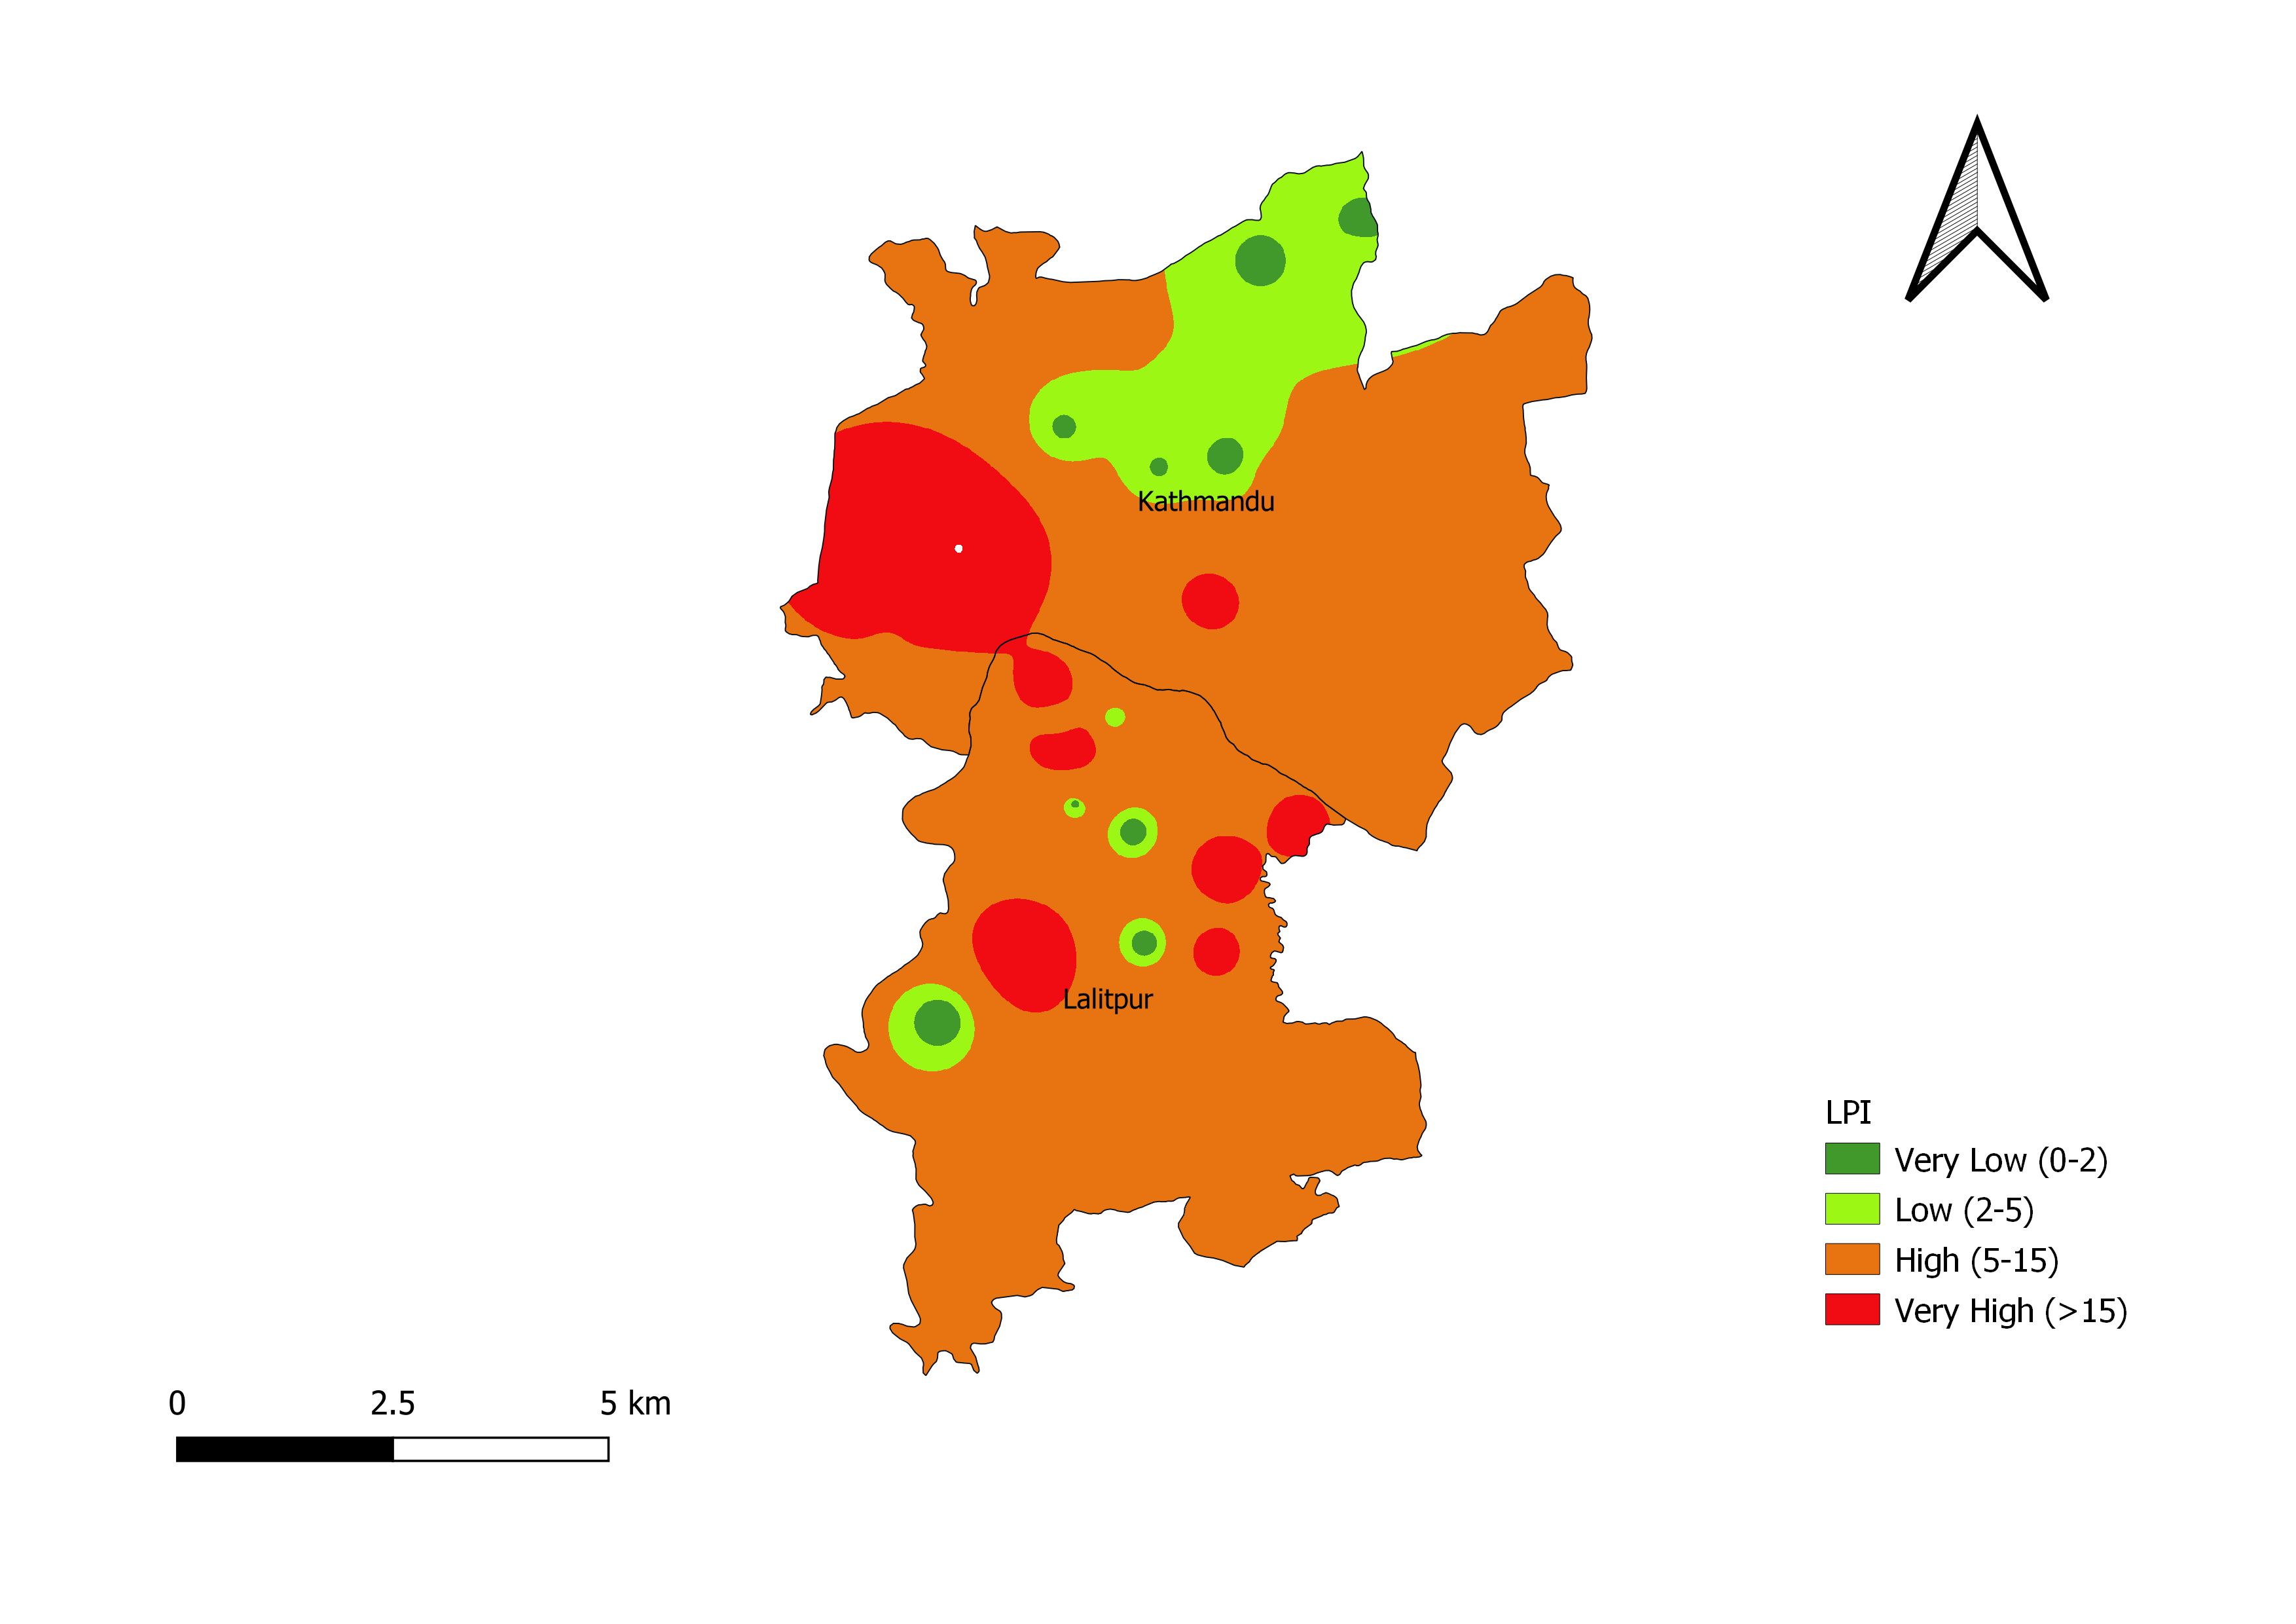
\includegraphics[width=0.8\linewidth, height=0.8\textheight,keepaspectratio]{in/map/LPI.png}
\caption{LPI}
\end{figure}
\pagebreak
\end{landscape}

\section{Summary for Area}
\textbf{Total Area:} 85546375.23 $m^2$\\
\begin{center}
\subsection{LPI}
\begin{tabular}{|c | c | c|} 
\hline
Liquefaction Potential & Area($m^2$) & \% \\
\hline
Very low & 1156807.604 & 1.352257885 \\
Low & 9528705.043 & 11.13864266 \\
High & 64499949.72 & 75.39764198 \\
Very High & 10360912.86 & 12.11145748 \\
\hline
\end{tabular}
\hfill

\subsection{Shear(1.5m)}
\begin{tabular}{|c | c | c|} 
\hline
Soil Type & Area($m^2$) & \% \\
\hline
Weak soil & 6373.329037	& 0.007450145 \\
Soft soil & 301298.4954	& 0.352204865 \\ 
Medium & 878072.0773	& 1.026428151 \\
Moderately hard & 2300390.906	& 2.689057134 \\
Hard & 82055748.03	& 95.91960829 \\
\hline
\end{tabular}

\subsection{Shear(3.0m)}
\begin{tabular}{|c | c | c|} 
\hline
Soil Type & Area($m^2$) & \% \\
\hline
Weak soil & 4164.246861 & 0.004867824 \\
Soft soil & 155524.4635 & 0.181801348 \\
Medium & 437474.4461 & 0.511388641 \\
Moderately hard & 819442.5286 & 0.957892753 \\
Hard & 84125277.15 & 98.33879802 \\
\hline
\end{tabular}

\subsection{Shear(4.5m)}
\begin{tabular}{|c | c | c|} 
\hline
Soil Type & Area($m^2$) & \% \\
\hline
Weak soil & 2843.875905	& 0.003324368 \\
Soft soil & 104410.8725	& 0.122051779 \\
Medium & 551153.307	& 0.644274296 \\
Moderately hard & 1246811.059 & 1.457468017 \\
Hard & 83636663.72 & 97.76763012 \\
\hline
\end{tabular}
\pagebreak

\subsection{Settlement(1.5m)}
\begin{tabular}{|c | c | c|} 
\hline
Soil Type & Area($m^2$) & \% \\
\hline
Weak soil & 2835547.411 & 3.314631863 \\
Soft soil & 19632951.23 & 22.95006793 \\
Medium & 46110603.92 & 53.90129482 \\
Moderately hard & 11795026.1 & 13.78787361 \\
Hard & 5167754.179 & 6.040880358 \\
\hline
\end{tabular}

\subsection{Settlement(3.0m)}
\begin{tabular}{|c | c | c|} 
\hline
Soil Type & Area($m^2$) & \% \\
\hline
Weak soil & 4475346.571 & 5.231485915 \\
Soft soil & 26164648.6 & 30.58533869 \\
Medium & 45074976.04 & 52.69069077 \\
Moderately hard & 6731174.957 & 7.868451398 \\
Hard & 3095736.665 & 3.618781808 \\
\hline
\end{tabular}

\subsection{Settlement(4.5m)}
\begin{tabular}{|c | c | c|} 
\hline
Soil Type & Area($m^2$) & \% \\
\hline
Weak soil & 10479251.05 & 12.24978969 \\
Soft soil & 54117790.45 & 63.26134836 \\
Medium & 18542807.26 & 21.67573694 \\
Moderately hard & 1598689.918 & 1.868799133 \\
Hard & 803344.1596 & 0.939074458 \\
\hline
\end{tabular}
\pagebreak

\subsection{Net Allowable(1.5m)}
\begin{tabular}{|c | c | c|} 
\hline
Soil Type & Area($m^2$) & \% \\
\hline
Weak soil & 4475616.392 & 5.231801324\\
Soft soil & 26166517.1 & 30.58752289\\
Medium & 45080608.34 & 52.69727468\\
Moderately hard & 6744721.273 & 7.884286452\\
Hard & 3079822.333 & 3.600178646\\
\hline
\end{tabular}

\subsection{Net Allowable(3.0m)}
\begin{tabular}{|c | c | c|} 
\hline
Soil Type & Area($m^2$) & \% \\
\hline
Weak soil & 2835619.316 & 3.314715916\\
Soft soil & 19634486.32 & 22.95186239\\
Medium & 46130780.34 & 53.92488018\\
Moderately hard & 11805693.59 & 13.80034345\\
Hard & 5140705.862 & 6.00926205\\
\hline
\end{tabular}

\subsection{Net Allowable(4.5m)}
\begin{tabular}{|c | c | c|} 
\hline
Soil Type & Area($m^2$) & \% \\
\hline
Weak soil & 10480085.37 & 12.25076496 \\
Soft soil & 54121503.26 & 63.26568849\\
Medium & 18543457.22 & 21.67649672\\
Moderately hard & 1598962.234 & 1.869117458\\
Hard & 803277.3478 & 0.938996358\\
\hline
\end{tabular}
\end{center}

\pagebreak

\section{Summary of Result from Various Methods}
\begin{table}[!h]
\caption{Methods summary Table}
\begin{tabularx}{\textwidth}{ | l | p{0.32\textwidth} | X | X | X | X | }
\hline
 \textbf{S.N.} & \textbf{Method} & \textbf{Mean($\overline{x}$)} & \textbf{Standard deviation ($\sigma$)} & \textbf{Minimum ($x_{min}$)} & \textbf{Minimum ($x_{min}$)}\\
\hline
 1 & \mbox{Terzaghi(1.5m)} & 273.165 & 195.294 & 68.073 & 853.968 \\
 2 & \mbox{Terzaghi(3.0m)} & 486.183 & 374.592 & 68.073 & 1586.820 \\
 3 & \mbox{Terzaghi(4.5m)} & 558.054 & 464.913 & 68.073 & 1978.576 \\
\hline
 4 & \mbox{Meyerhof(1.5m)} & 318.623 & 261.939 & 65.041 & 1026.956 \\
 5 & \mbox{Meyerhof(3.0m)} & 682.630 & 569.958 & 73.525 & 2190.626 \\
 6 & \mbox{Meyerhof(4.5m)} & 853.622 & 756.113 & 82.008 & 3197.508 \\
\hline
 7 & \mbox{Hansen(1.5m)} & 352.225 & 267.698 & 78.817 & 1143.045 \\
 8 & \mbox{Hansen(3.0m)} & 773.252 & 631.410 & 78.817 & 2498.216 \\
 9 & \mbox{Hansen(4.5m)} & 1039.835 & 944.778 & 78.817 & 3827.666 \\
\hline
 10 & \mbox{Vesic(1.5m)} & 366.964 & 285.722 & 78.817 & 1223.801 \\
 11 & \mbox{Vesic(3.0m)} & 791.445 & 650.804 & 78.817 & 2584.092 \\
 12 & \mbox{Vesic(4.5m)} & 1054.421 & 960.962 & 78.817 & 3888.722 \\
\hline
 13 & \mbox{Plaxis Shear(1.5m)} & 388.225 & 310.462 & 21.890 & 1191.875 \\
 14 & \mbox{Plaxis Shear(3.0m)} & 563.378 & 470.487 & 105.480 & 1984.930 \\
 15 & \mbox{Plaxis Shear(4.5m)} & 738.074 & 626.830 & 120.814 & 2244.375 \\
\hline
 16 & \mbox{Teng Shear(1.5m)} & 153.173 & 93.268 & 52.903 & 461.283 \\
 17 & \mbox{Teng Shear(3.0m)} & 346.263 & 245.070 & 94.750 & 1055.146 \\
 18 & \mbox{Teng Shear(4.5m)} & 450.276 & 268.759 & 129.275 & 1231.453 \\
\hline
 19 & \mbox{Bowels(1.5m)} & 217.306 & 128.281 & 43.732 & 612.250 \\
 20 & \mbox{Bowels(3.0m)} & 216.309 & 131.719 & 52.400 & 592.947 \\
 21 & \mbox{Bowels(4.5m)} & 178.876 & 95.570 & 54.671 & 452.777 \\
\hline
 22 & \mbox{Peck(1.5m)} & 151.702 & 91.971 & 31.946 & 412.740 \\
 23 & \mbox{Peck(3.0m)} & 141.799 & 83.494 & 32.672 & 359.938 \\
 24 & \mbox{Peck(4.5m)} & 122.204 & 66.145 & 33.091 & 277.131 \\
\hline
 25 & \mbox{Teng Settlement(1.5m)} & 165.761 & 126.774 & -16.572 & 557.774 \\
 26 & \mbox{Teng Settlement(3.0m)} & 185.825 & 141.252 & 3.668 & 581.152 \\
 27 & \mbox{Teng Settlement(4.5m)} & 151.782 & 101.696 & 11.532 & 464.391 \\
\hline
 28 & \mbox{Plaxis Settlement(1.5m)} & 64.355 & 19.113 & 35.110 & 111.952 \\
 29 & \mbox{Plaxis Settlement(3.0m)} & 68.618 & 14.859 & 40.915 & 107.151 \\
 30 & \mbox{Plaxis Settlement(4.5m)} & 76.632 & 18.282 & 47.316 & 128.371 \\
\hline
 31 & \mbox{Meyerhof Settlement(1.5m)} & 144.871 & 85.521 & 29.155 & 408.167 \\
 32 & \mbox{Meyerhof Settlement(3.0m)} & 144.206 & 87.813 & 34.933 & 395.298 \\
 33 & \mbox{Meyerhof Settlement(4.5m)} & 119.250 & 63.713 & 36.448 & 301.851 \\
\hline
\end{tabularx}

\end{table}
\pagebreak

\section{Correlation and regression between methods}
\subsection{Terzaghi}
\begin{tabularx}{\textwidth}{ | p{0.32\textwidth} | X | X | }
\hline
\textbf{Method(x)} & \textbf{Correlation} & \textbf{Regression} \\
\hline
 Meyerhof & 0.9961 & 0.5746 x + 71.0810\\
 Hansen & 0.9834 & 0.5368 x + 61.5623\\
 Vesic & 0.9862 & 0.5262 x + 60.1358\\
 Plaxis Shear & 0.3230 & 0.2980 x + 315.0004\\
 Teng Shear & 0.6134 & 0.7774 x + 175.1218\\
 Bowels & 0.4626 & 1.2177 x + 191.7191\\
 Peck & 0.4195 & 1.7164 x + 215.3036\\
 Teng Settlement & 0.4887 & 1.2721 x + 226.9952\\
 Plaxis Settlement & 0.4708 & 10.0284 x  -238.9545\\
 Meyerhof Settlement & 0.4626 & 1.8265 x + 191.7191\\
\hline
\end{tabularx}
\subsection{Meyerhof}
\begin{tabularx}{\textwidth}{ | p{0.32\textwidth} | X | X | }
\hline
\textbf{Method(x)} & \textbf{Correlation} & \textbf{Regression} \\
\hline
 Terzaghi & 0.9961 & 1.7266 x  -117.0397\\
 Hansen & 0.9867 & 0.9337 x  -16.1185\\
 Vesic & 0.9888 & 0.9145 x  -18.1031\\
 Plaxis Shear & 0.3068 & 0.4907 x + 440.4858\\
 Teng Shear & 0.6224 & 1.3674 x + 175.2632\\
 Bowels & 0.4544 & 2.0735 x + 220.9309\\
 Peck & 0.4075 & 2.8903 x + 266.2143\\
 Teng Settlement & 0.4813 & 2.1716 x + 279.8926\\
 Plaxis Settlement & 0.4789 & 17.6807 x  -556.0667\\
 Meyerhof Settlement & 0.4544 & 3.1103 x + 220.9309\\
\hline
\end{tabularx}
\subsection{Hansen}
\begin{tabularx}{\textwidth}{ | p{0.32\textwidth} | X | X | }
\hline
\textbf{Method(x)} & \textbf{Correlation} & \textbf{Regression} \\
\hline
 Terzaghi & 0.9834 & 1.8014 x  -84.8532\\
 Meyerhof & 0.9867 & 1.0427 x + 37.7142\\
 Vesic & 0.9998 & 0.9772 x  -0.2805\\
 Plaxis Shear & 0.3349 & 0.5659 x + 465.9312\\
 Teng Shear & 0.5797 & 1.3458 x + 252.3916\\
 Bowels & 0.3820 & 1.8421 x + 345.3049\\
 Peck & 0.3342 & 2.5044 x + 395.5045\\
 Teng Settlement & 0.4125 & 1.9667 x + 390.0802\\
 Plaxis Settlement & 0.4425 & 17.2650 x  -457.5097\\
 Meyerhof Settlement & 0.3820 & 2.7632 x + 345.3049\\
\hline
\end{tabularx}
\subsection{Vesic}
\begin{tabularx}{\textwidth}{ | p{0.32\textwidth} | X | X | }
\hline
\textbf{Method(x)} & \textbf{Correlation} & \textbf{Regression} \\
\hline
 Terzaghi & 0.9862 & 1.8484 x  -88.9498\\
 Meyerhof & 0.9888 & 1.0692 x + 37.3341\\
 Hansen & 0.9998 & 1.0230 x + 0.5485\\
 Plaxis Shear & 0.3339 & 0.5773 x + 478.1299\\
 Teng Shear & 0.5838 & 1.3867 x + 254.7966\\
 Bowels & 0.3914 & 1.9311 x + 342.5569\\
 Peck & 0.3445 & 2.6417 x + 392.6198\\
 Teng Settlement & 0.4212 & 2.0550 x + 390.8499\\
 Plaxis Settlement & 0.4451 & 17.7686 x  -475.1583\\
 Meyerhof Settlement & 0.3914 & 2.8967 x + 342.5569\\
\hline
\end{tabularx}
\subsection{Plaxis Shear}
\begin{tabularx}{\textwidth}{ | p{0.32\textwidth} | X | X | }
\hline
\textbf{Method(x)} & \textbf{Correlation} & \textbf{Regression} \\
\hline
 Terzaghi & 0.3230 & 0.3502 x + 402.4522\\
 Meyerhof & 0.3068 & 0.1919 x + 434.0758\\
 Hansen & 0.3349 & 0.1982 x + 415.9656\\
 Vesic & 0.3339 & 0.1931 x + 416.3466\\
 Teng Shear & -0.0620 & -0.0852 x + 606.5472\\
 Bowels & -0.0989 & -0.2821 x + 640.5997\\
 Peck & -0.0373 & -0.1656 x + 598.5786\\
 Teng Settlement & -0.0923 & -0.2605 x + 625.4717\\
 Plaxis Settlement & 0.0833 & 1.9246 x + 433.4478\\
 Meyerhof Settlement & -0.0989 & -0.4232 x + 640.5997\\
\hline
\end{tabularx}
\subsection{Teng Shear}
\begin{tabularx}{\textwidth}{ | p{0.32\textwidth} | X | X | }
\hline
\textbf{Method(x)} & \textbf{Correlation} & \textbf{Regression} \\
\hline
 Terzaghi & 0.6134 & 0.4840 x + 164.3791\\
 Meyerhof & 0.6224 & 0.2833 x + 195.0166\\
 Hansen & 0.5797 & 0.2497 x + 202.1657\\
 Vesic & 0.5838 & 0.2457 x + 200.6771\\
 Plaxis Shear & -0.0620 & -0.0452 x + 425.2438\\
 Bowels & 0.8469 & 1.7591 x  -25.1633\\
 Peck & 0.7514 & 2.4256 x + 17.4066\\
 Teng Settlement & 0.8800 & 1.8073 x + 31.9734\\
 Plaxis Settlement & 0.5923 & 9.9545 x  -319.8311\\
 Meyerhof Settlement & 0.8469 & 2.6386 x  -25.1633\\
\hline
\end{tabularx}
\subsection{Bowels}
\begin{tabularx}{\textwidth}{ | p{0.32\textwidth} | X | X | }
\hline
\textbf{Method(x)} & \textbf{Correlation} & \textbf{Regression} \\
\hline
 Terzaghi & 0.4626 & 0.1757 x + 156.0270\\
 Meyerhof & 0.4544 & 0.0996 x + 169.5154\\
 Hansen & 0.3820 & 0.0792 x + 178.7789\\
 Vesic & 0.3914 & 0.0793 x + 177.2090\\
 Plaxis Shear & -0.0989 & -0.0346 x + 261.1880\\
 Teng Shear & 0.8469 & 0.4077 x + 78.5048\\
 Peck & 0.9262 & 1.4395 x + 14.6612\\
 Teng Settlement & 0.9961 & 0.9849 x + 41.1175\\
 Plaxis Settlement & 0.5438 & 4.4000 x  -76.5516\\
 Meyerhof Settlement & 1.0000 & 1.5000 x + 0.0000\\
\hline
\end{tabularx}
\subsection{Peck}
\begin{tabularx}{\textwidth}{ | p{0.32\textwidth} | X | X | }
\hline
\textbf{Method(x)} & \textbf{Correlation} & \textbf{Regression} \\
\hline
 Terzaghi & 0.4195 & 0.1025 x + 107.6899\\
 Meyerhof & 0.4075 & 0.0575 x + 116.0278\\
 Hansen & 0.3342 & 0.0446 x + 122.2639\\
 Vesic & 0.3445 & 0.0449 x + 121.1565\\
 Plaxis Shear & -0.0373 & -0.0084 x + 162.3026\\
 Teng Shear & 0.7514 & 0.2328 x + 64.5187\\
 Bowels & 0.9262 & 0.5959 x + 13.6502\\
 Teng Settlement & 0.9161 & 0.5828 x + 38.9951\\
 Plaxis Settlement & 0.5052 & 2.6305 x  -32.5722\\
 Meyerhof Settlement & 0.9262 & 0.8939 x + 13.6502\\
\hline
\end{tabularx}
\subsection{Teng Settlement}
\begin{tabularx}{\textwidth}{ | p{0.32\textwidth} | X | X | }
\hline
\textbf{Method(x)} & \textbf{Correlation} & \textbf{Regression} \\
\hline
 Terzaghi & 0.4887 & 0.1878 x + 112.1201\\
 Meyerhof & 0.4813 & 0.1067 x + 126.3406\\
 Hansen & 0.4125 & 0.0865 x + 134.9648\\
 Vesic & 0.4212 & 0.0863 x + 133.4767\\
 Plaxis Shear & -0.0923 & -0.0327 x + 222.0370\\
 Teng Shear & 0.8800 & 0.4285 x + 32.1555\\
 Bowels & 0.9961 & 1.0075 x  -39.8615\\
 Peck & 0.9161 & 1.4400 x  -23.4806\\
 Plaxis Settlement & 0.5551 & 4.5429 x  -124.9285\\
 Meyerhof Settlement & 0.9961 & 1.5112 x  -39.8615\\
\hline
\end{tabularx}
\subsection{Plaxis Settlement}
\begin{tabularx}{\textwidth}{ | p{0.32\textwidth} | X | X | }
\hline
\textbf{Method(x)} & \textbf{Correlation} & \textbf{Regression} \\
\hline
 Terzaghi & 0.4708 & 0.0221 x + 61.5182\\
 Meyerhof & 0.4789 & 0.0130 x + 62.8954\\
 Hansen & 0.4425 & 0.0113 x + 63.2938\\
 Vesic & 0.4451 & 0.0111 x + 63.2368\\
 Plaxis Shear & 0.0833 & 0.0036 x + 70.1845\\
 Teng Shear & 0.5923 & 0.0352 x + 58.1759\\
 Bowels & 0.5438 & 0.0672 x + 56.0315\\
 Peck & 0.5052 & 0.0970 x + 56.9684\\
 Teng Settlement & 0.5551 & 0.0678 x + 58.4611\\
 Meyerhof Settlement & 0.5438 & 0.1008 x + 56.0315\\
\hline
\end{tabularx}
\subsection{Meyerhof Settlement}
\begin{tabularx}{\textwidth}{ | p{0.32\textwidth} | X | X | }
\hline
\textbf{Method(x)} & \textbf{Correlation} & \textbf{Regression} \\
\hline
 Terzaghi & 0.4626 & 0.1171 x + 104.0180\\
 Meyerhof & 0.4544 & 0.0664 x + 113.0102\\
 Hansen & 0.3820 & 0.0528 x + 119.1859\\
 Vesic & 0.3914 & 0.0529 x + 118.1394\\
 Plaxis Shear & -0.0989 & -0.0231 x + 174.1253\\
 Teng Shear & 0.8469 & 0.2718 x + 52.3366\\
 Bowels & 1.0000 & 0.6667 x + 0.0000\\
 Peck & 0.9262 & 0.9596 x + 9.7741\\
 Teng Settlement & 0.9961 & 0.6566 x + 27.4117\\
 Plaxis Settlement & 0.5438 & 2.9333 x  -51.0344\\
\hline
\end{tabularx}
